\documentclass[stu, 12pt, letterpaper, donotrepeattitle, floatsintext, natbib]{apa7}
\usepackage[utf8]{inputenc}
\usepackage[T1]{fontenc}
\usepackage{adjustbox}
\usepackage{longtable}
\usepackage{tabularx}
\usepackage{lmodern}
\usepackage{comment}
\usepackage{marvosym}
\usepackage{graphicx}
\usepackage{float}
\usepackage[normalem]{ulem}
\usepackage[spanish]{babel}
\usepackage{multirow}
\usepackage{tabularx}
\usepackage{tabularray}
\usepackage{adjustbox}
\usepackage{geometry}
\usepackage{tikz}
\usepackage{enumitem}
\usepackage{hyperref}
\usepackage{amsmath}
\usepackage{pgfgantt}
\usepackage{apacite}
\usepackage{array}
\usepackage{pdfpages}

\usetikzlibrary{shapes.geometric, arrows, positioning, fit, calc}
\selectlanguage{spanish}
\useunder{\uline}{\ul}{}
\newcommand{\myparagraph}[1]{\paragraph{#1}\mbox{}\\}

% Portada
\title{\Large Plan de Pruebas}
\author{
    Campero Morales José Antonio \\
    Campohermoso Berdeja Oscar \\
    Carrasco Cespedes Miguel Alejandro \\
    Martinez Acarapi Fabiola Alejandra \\
    Montero Garrido Diana Aneliz \\
    Zizold Sempertegui Gabriela Zulema Britta
}
\affiliation{Universidad Católica Boliviana}
\course{SIS-312: Gestión de Calidad de Sistemas}
\professor{Lic. Cecilia Alvarado Monrroy}
\duedate{\textbf{15 de diciembre de 2024}}

\newcommand{\userstory}[5]{ % Change from 4 to 5 arguments
    \begin{center}
        \begin{tikzpicture}
            \node[draw, rounded corners, fill=blue!10, text width=0.9\textwidth, align=center, inner sep=10pt] {
                \textbf{#1} \\[5pt]
                \textit{Como} #2, \\[5pt]
                \textit{quiero} #3 \\[5pt]
                \textit{para} #4 \\[5pt]
                \href{#5}{Ver en GitHub} 
            };
        \end{tikzpicture}
    \end{center}
    \vspace{10pt}
}

\begin{document}
\thispagestyle{empty}

% Add the logo before the title content, avoiding extra space
\centering

\includegraphics[width=0.8\textwidth]{../imgs/logo-ucb.png} % Adjust the path to your logo image
\vspace{-5cm} % Adjust negative space if needed

\maketitle

% Índices
\newpage
\pagenumbering{roman}
% Contenido
\renewcommand\contentsname{\large Índice}
\tableofcontents
\setcounter{tocdepth}{2}
\newpage
% Fíguras
\renewcommand{\listfigurename}{\large Índice de figuras}
\listoffigures
\newpage
% Tablas
\renewcommand{\listtablename}{\large Índice de tablas}
\listoftables
\newpage

% Cuerpo
\pagenumbering{arabic}
\section{\large Introducci\'on}

\noindent Este plan de pruebas tiene como objetivo definir y organizar las actividades de prueba para los m\'odulos principales de la aplicaci\'on \textit{Bajo Esquina}. Esta aplicaci\'on es un editor de grafos que ofrece una variedad de herramientas avanzadas para la creaci\'on, manipulaci\'on y an\'alisis de estructuras de grafos, as\'i como funcionalidades orientadas a la resoluci\'on de problemas reales en el \'ambito de los grafos y las estructuras de datos.

\noindent Entre sus caracter\'isticas destacadas, la aplicaci\'on incluye un m\'odulo optimizado para calcular rutas \'optimas en la red de telef\'ericos de la ciudad de La Paz, Bolivia. Este m\'odulo est\'a dise\~nado para ayudar a los usuarios a optimizar trayectos considerando criterios como costo y tiempo. Adem\'as, la aplicaci\'on incluye diversas funcionalidades para la generaci\'on de grafos personalizados, la representaci\'on de matrices de adyacencia y costos, y una interfaz amigable para facilitar la interacci\'on con sus herramientas.

\noindent El prop\'osito de este plan de pruebas es asegurar que los m\'odulos desarrollados de distintos algoritmos implementados cumplan con los requisitos funcionales, ofrezcan una experiencia de usuario fluida y proporcionen resultados precisos y eficientes. Este enfoque busca garantizar la calidad del sistema mediante pruebas que eval\'uen su funcionalidad, robustez y usabilidad, asegurando que cumpla con los objetivos establecidos y satisfaga las expectativas de los usuarios finales.

% \noindent El \textit{editor Northwest}, uno de los editores desarrollados, está diseñado específicamente para el método de la esquina noroeste (\textit{Northwest Corner Method}), una técnica utilizada para resolver problemas de transporte y asignación de recursos. Este método ofrece una solución inicial factible al distribuir suministros y demandas de manera efectiva, lo cual facilita la posterior optimización del costo total de transporte.

% \noindent La elección de este editor para el plan de pruebas responde al interés de explorar cómo este algoritmo puede generar soluciones iniciales basadas en condiciones específicas de oferta y demanda. Además, el editor Northwest permite la manipulación visual de grafos y la generación de la matriz de adyacencia, convirtiéndolo en una herramienta práctica tanto para el análisis como para la resolución de problemas de asignación. A continuación, se presenta un plan de pruebas para asegurar la funcionalidad completa y la robustez del editor Northwest.

\subsection{Alcance del Plan de Pruebas}

El presente plan de pruebas plantea evaluar de manera integral el sistema desarrollado, abarcando múltiples módulos y funcionalidades clave, con el fin de garantizar su correcto funcionamiento, accesibilidad, usabilidad y cumplimiento de los objetivos especificados. A continuación, se detallan los alcances específicos de las pruebas:

\subsubsection{Áreas incluidas en las pruebas}

\begin{itemize}
    \item \textbf{Creación y visualización de grafos:} Se evaluará la capacidad del editor para permitir la creación precisa de grafos, incluyendo la adición, edición y conexión de nodos y aristas, asegurando que los grafos generados se representen de manera adecuada en el entorno gráfico del editor.
    
    \item \textbf{Guardado y carga de grafos:} Se comprobará que los datos de los grafos se almacenen y recuperen correctamente, permitiendo la continuidad del análisis y la manipulación en futuras sesiones.

    \item \textbf{Generación de matrices:} Las pruebas cubrirán:
    \begin{itemize}
        \item \textbf{Matriz de adyacencia:} Verificar que refleje con precisión las conexiones y relaciones entre los nodos del grafo.
        \item \textbf{Matriz de costos:} Evaluar su construcción precisa basada en los nodos y sus conexiones, garantizando que represente correctamente las relaciones de costos entre puntos de suministro y demanda.
    \end{itemize}

    \item \textbf{Optimización:} Se revisará la funcionalidad del módulo de optimización, asegurando que pueda resolver problemas de maximización y minimización de manera consistente con los objetivos definidos.

    \item \textbf{Interfaz de usuario y usabilidad:} Se evaluará la facilidad de uso y la accesibilidad de la interfaz desarrollada en Vue.js, evaluando que cumpla con los criterios de accesibilidad de la WCAG versión 2.2 y que los resultados del sistema sean presentados de forma clara y comprensible para los usuarios.

    \item \textbf{Algoritmos implementados:} Se evaluará la correcta ejecución y funcionalidad de los siguientes algoritmos:
    \begin{itemize}
        \item \textbf{Algoritmo de Asignación:} Incluyendo la interacción entre el backend en Spring Boot y la base de datos MySQL, para garantizar que los datos se almacenen y recuperen adecuadamente.
        \item \textbf{Compet:} Se verificará la funcionalidad de su dashboard de edición de grafos, permitiendo la adición de nodos y la resolución eficiente del algoritmo mediante accesos directos.
        \item \textbf{Dijkstra:} Se evaluarán opciones avanzadas como la selección de nodos inicial y destino, así como la ejecución del algoritmo para minimizar o maximizar rutas.
        \item \textbf{Kruskal:} Verificación de la implementación y resultados del algoritmo en el contexto del sistema de gestión de grafos.
        \item \textbf{Algoritmo de Johnson:} Se comprobará la correcta implementación del algoritmo para resolver problemas de caminos más cortos en grafos dirigidos con otras funcionalidades del editor.
        \item \textbf{Método de la esquina noroeste (North-West):} Se evaluará su capacidad para resolver problemas de transporte, verificando que las soluciones iniciales se calculen correctamente y se representen de manera adecuada en las matrices de costos.
        \item \textbf{Sorts:} Evaluar la ejecución de los algoritmos de ordenamiento (Selection Sort, Insertion Sort, Merge Sort, Shell Sort), verificando la correcta representación del proceso y su animación a diferentes velocidades.
        \item \textbf{Árboles Binarios:} Se probará la creación, visualización gráfica y recorridos (inorden, preorden, postorden) de los árboles binarios, garantizando que los datos se representen adecuadamente.
    \end{itemize}

        
\end{itemize}

\subsubsection{Áreas excluidas de las pruebas}

\begin{itemize}
    \item \textbf{Componentes externos al editor:} No se evaluarán funcionalidades relacionadas con la manipulación de archivos de grafos creados previamente o la descripción del algoritmo en la interfaz inicial, ya que se consideran fuera del alcance del editor.
    
    \item \textbf{Pruebas de estrés:} No se realizarán pruebas de desempeño bajo condiciones extremas de carga en esta fase del proyecto. Estas evaluaciones serán consideradas para iteraciones futuras.
\end{itemize}


\subsection{Objetivos}

\subsubsection{Objetivo General}
Garantizar la correcta funcionalidad, usabilidad y calidad de los diferentes módulos y algoritmos implementados en el sistema, validando que cumplan con las especificaciones técnicas y funcionales definidas, y que proporcionen una experiencia de usuario eficiente y minimizando de errores.

\subsubsection{Objetivos Específicos}

\begin{itemize}
    \item Validar la precisión y correcta ejecución de los algoritmos implementados, asegurando resultados optimizados y libres de errores.
    \item Comprobar que la interfaz de usuario desarrollada en Vue.js sea accesible, intuitiva y cumpla con los estándares de accesibilidad WCAG 2.2.
    \item Confirmar la integración precisa y estable entre los componentes del sistema, como la interfaz, el backend y la base de datos.
    \item Detectar y documentar errores o áreas de mejora en el sistema, permitiendo su corrección antes de la implementación en producción.
    \item Validar la funcionalidad de módulos específicos, como el editor de grafos y la gestión de estructuras de datos, asegurando su correcto desempeño.
    \item Evaluar la experiencia del usuario, garantizando una interacción fluida, estable y libre de errores críticos o caídas inesperadas.
\end{itemize}


\subsection{Limitaciones}

El presente plan de pruebas contempla diversas limitaciones que restringen el alcance y el entorno en el cual se ejecutarán las pruebas. A continuación, se describen dichas limitaciones:

\begin{itemize}
    \item \textbf{Datos de prueba limitados:} La disponibilidad de datos de prueba representativos es limitada, lo que podría restringir la validación a configuraciones específicas de oferta y demanda, dejando fuera algunos escenarios posibles que podrían presentarse en situaciones reales. Además, los datos de prueba utilizados son simulados y pueden no representar la diversidad de datos procesados en producción.

    \item \textbf{Entorno de pruebas no desplegado:} Las pruebas se realizarán en un entorno de desarrollo, sin acceso a un ambiente de staging ni a una instancia de deploy. Por lo tanto, los resultados pueden no reflejar completamente el rendimiento o la experiencia de usuario final en un entorno de producción. Esto también implica que no se realizarán pruebas de carga, estrés o escalabilidad a gran escala.

    \item \textbf{Exclusión de componentes específicos:} Los contenedores de \textit{Keycloak}, \textit{MinIO} y \textit{Python} no serán objeto de pruebas directas. Sin embargo, cualquier incidencia en su funcionamiento que afecte a los módulos bajo prueba será documentada.

    \item \textbf{Funcionalidades no finalizadas:} Algunas funcionalidades del sistema están en etapas de desarrollo o modificación, como la autenticación con Google. Estas características no serán evaluadas en las pruebas actuales debido a su estado de implementación.

    \item \textbf{Pruebas de rendimiento excluidas:} No se realizarán pruebas de rendimiento o de carga a gran escala debido a las limitaciones del entorno de desarrollo. Las pruebas de rendimiento deberán ejecutarse en un entorno de staging o producción para garantizar su validez.

    \item \textbf{Pruebas de seguridad excluidas:} Este plan no contempla evaluaciones sobre la gestión de autenticación, autorización, cifrado de datos ni posibles vulnerabilidades de seguridad. Estas pruebas deben ser consideradas en futuros planes de validación.

    \item \textbf{Limitaciones en funcionalidades del frontend:} Las pruebas funcionales en el frontend estarán limitadas a verificar la interacción del \textit{dashboard} de nodos y arcos con los algoritmos de \textit{Compet} y \textit{Dijkstra}. Otras funcionalidades del \textit{dashboard} y la interfaz de usuario no serán evaluadas.

    \item \textbf{Compatibilidad limitada de accesibilidad:} Las pruebas de accesibilidad se limitarán a elementos básicos, como la navegación con teclado y el contraste visual en componentes relacionados con los algoritmos de \textit{Compet} y \textit{Dijkstra}. No se evaluarán estándares adicionales de accesibilidad en otros módulos.
\end{itemize}


\subsection{Base de la Prueba}
\subsubsection{Descripción del Sistema}
El proyecto "Bajo Esquina" es un sistema web que permite a los usuarios crear, editar y visualizar grafos, así como realizar análisis a través de algoritmos clave en el ámbito de la teoría de grafos. Los usuarios pueden interactuar con el sistema a través de un editor visual, el cual les permite construir grafos al agregar, modificar o eliminar nodos y aristas.

\noindent El objetivo es ofrecer una plataforma que no solo facilite la creación y manipulación de grafos, sino que también permita aplicar algoritmos relevantes, manteniendo la integridad y precisión en los cálculos y la representación visual. Este sistema está diseñado para estudiantes, profesionales y cualquier usuario interesado en la teoría de grafos y su aplicación práctica, brindando una experiencia de usuario interactiva, intuitiva y funcional.

\subsubsection{Requisitos del Sistema}
Los requisitos del sistema definen las necesidades y expectativas que los distintos módulos del sistema deben cumplir para asegurar una funcionalidad completa y efectiva. Estos incluyen:

\begin{itemize}
    \item \textbf{Creación de cuentas y acceso seguro}:  
    Los usuarios deberán poder realizar la creación de cuentas personales vinculando su cuenta a un correo electrónico y una contraseña segura, así como deberán poder acceder al sistema mediante un inicio de sesión seguro que gestione credenciales. 

    \item \textbf{Creación y visualización de grafos}: 
    El editor deberá permitir a los usuarios crear grafos, incluyendo la adición de nodos y aristas, y visualizar los grafos de forma clara e intuitiva dentro de la interfaz del editor.

    \item \textbf{Carga y descarga de grafos}: 
    El editor permitirá a los usuarios cargar grafos guardados desde su computador y descargar los grafos creados para su almacenamiento local, asegurando que la información se maneje de forma precisa y sin pérdidas.

    \item \textbf{Generación automática de la matriz de adyacencia}: 
    A partir de los grafos creados en el editor, este deberá generar automáticamente una matriz de adyacencia que refleje correctamente las conexiones entre los nodos definidos.

    \item \textbf{Generación automática de la matriz de costos}: 
    El editor deberá generar de manera automática una matriz de costos basada en los nodos y conexiones definidas por el usuario, asegurando que la información de costos esté alineada con los datos ingresados.

    \item \textbf{Manejo de oferta y demanda}: 
    El editor deberá gestionar situaciones donde la oferta y la demanda no estén balanceadas. Si es necesario, ajustará automáticamente las configuraciones para asegurar que no se produzcan errores en los cálculos de transporte.

    \item \textbf{Funcionalidades de optimización}: 
    El editor deberá ofrecer opciones que permitan al usuario seleccionar entre maximización o minimización de soluciones, proporcionando resultados válidos y ajustados a los objetivos especificados en las configuraciones de entrada.

    \item \textbf{Resolución de grafos complejos}:
    El editor deberá proporcionar herramientas avanzadas para resolver grafos con características complejas, como valores extremos o negativos, y múltiples relaciones. Los algoritmos implementados deberán manejar estas condiciones sin generar errores, asegurando que los resultados sean precisos y comprensibles. Además, el sistema deberá notificar al usuario si los datos ingresados no son válidos para el análisis.

    \item \textbf{Visualización interactiva de procesos de ordenamiento}:
    El editor deberá permitir a los usuarios observar de manera interactiva el proceso de ordenamiento de listas de datos. La visualización debe mostrar cada paso del algoritmo en tiempo real, permitiendo ajustar la velocidad según las preferencias del usuario. 

    \item \textbf{Construcción y visualización de árboles binarios}:
    El editor deberá permitir a los usuarios construir árboles binarios mediante la inserción de nodos con valores definidos. Además, ofrecerá la visualización gráfica de la estructura del árbol, mostrando claramente sus niveles, conexiones y jerarquías. También deberá proporcionar opciones para realizar y mostrar recorridos preorden, inorden y postorden, asegurando que los datos se presenten de manera precisa y comprensible para el usuario.

    \item \textbf{Resolución de problemas de asignación}:
    El editor deberá permitir a los usuarios resolver problemas de asignación óptima mediante el uso de matrices de asignación. Los usuarios podrán definir manualmente o cargar los datos necesarios, y seleccionar criterios de maximización o minimización para obtener soluciones óptimas.
    
    \item \textbf{Accesibilidad del editor}: 
    Aunque no se ha pensado en un nivel profundo de accesibilidad, se espera que el editor, como mínimo, tenga un buen contraste de colores y cumpla con un nivel básico de accesibilidad.
\end{itemize}


\subsubsection{Especificaciones Funcionales}

Estas especificaciones detallan cada función del distintos editores y el comportamiento esperado, proporcionando instrucciones claras para los desarrolladores:

\begin{itemize}
    \item \textbf{Creación de cuentas y acceso seguro}:
    \begin{itemize}
    \item \textbf{Función}: Gestión de cuentas de usuario y accesos.
    \item \textbf{Requisitos funcionales}:
        \begin{itemize}
            \item Los usuarios deberán poder registrarse proporcionando un nombre de usuario, un correo electrónico y contraseña segura.
            \item El acceso al sistema deberá estar protegido por un inicio de sesión que gestione las credenciales de los usuarios.
        \end{itemize}
    \item \textbf{Proceso}:
        \begin{itemize}
            \item Los usuarios podrán registrarse o iniciar sesión a través de una interfaz segura.
        \end{itemize}
    \end{itemize}
    \item \textbf{Creación y visualización de grafos}:
    \begin{itemize}
        \item \textbf{Función}: Permitir la creación y visualización de grafos.
        \item \textbf{Requisitos funcionales}:
            \begin{itemize}
                \item El editor deberá permitir a los usuarios definir nodos y conexiones con pesos dentro del editor.
                \item Los grafos creados deben ser visualizados de forma intuitiva en la interfaz gráfica del editor.
                \item Se notificará al usuario si hay inconsistencias en la entrada de datos para asegurar la precisión en la creación del grafo.
            \end{itemize}
        \item \textbf{Proceso}:
            \begin{itemize}
                \item Al definir nodos y conexiones, el editor mostrará visualmente el grafo en tiempo real.
                \item Cualquier cambio en los nodos o aristas reflejará una actualización inmediata en la visualización.
            \end{itemize}
    \end{itemize}

    \item \textbf{Carga y descarga de grafos}:
    \begin{itemize}
        \item \textbf{Función}: Permitir la carga de grafos desde el computador y la descarga de grafos creados en el editor.
        \item \textbf{Requisitos funcionales}:
            \begin{itemize}
                \item El editor deberá permitir al usuario cargar grafos guardados en su computador en formato JSON, para que preserve toda la información de los nodos y conexiones.
                \item El editor deberá permitir al usuario descargar los grafos creados en formato JSON, garantizando así su integridad y que se puedan volver a cargar sin pérdida de 
                \item El editor deberá notificar al usuario sobre el estado de carga y descarga, indicando si estas operaciones se realizaron con éxito o si se presentaron problemas.
            \end{itemize}
        \item \textbf{Proceso}:
            \begin{itemize}
                \item El usuario podrá cargar grafos guardados en su computador en cualquier momento y descargará grafos generados para su almacenamiento local.
            \end{itemize}
    \end{itemize}


    \item \textbf{Generación de la matriz de adyacencia}:
    \begin{itemize}
        \item \textbf{Función}: Generación automática de la matriz de adyacencia a partir del grafo.
        \item \textbf{Requisitos funcionales}:
            \begin{itemize}
                \item El editor deberá calcular automáticamente la matriz de adyacencia que refleje las conexiones entre los nodos del grafo.
                \item El editor deberá permitir al usuario visualizar la matriz de adyacencia generada.
            \end{itemize}
        \item \textbf{Proceso}:
            \begin{itemize}
                \item Una vez creado el grafo, el editor generará automáticamente la matriz de adyacencia y permitirá su visualización al usuario.
                \item La matriz de adyacencia deberá reflejar correctamente las relaciones entre los nodos y las conexiones.
            \end{itemize}
    \end{itemize}

    \item \textbf{Generación de la matriz de costos}:
    \begin{itemize}
        \item \textbf{Función}: Generación automática de la matriz de costos basada en los pesos de las conexiones.
        \item \textbf{Requisitos funcionales}:
            \begin{itemize}
                \item El editor deberá permitir al usuario definir nodos y conexiones con pesos.
                \item El editor calculará la matriz de costos utilizando los valores de los pesos de las conexiones.
                \item La matriz de costos deberá reflejar correctamente las relaciones entre los puntos de suministro y demanda.
            \end{itemize}
        \item \textbf{Proceso}:
            \begin{itemize}
                \item Al definir nodos y conexiones, el editor generará automáticamente la matriz de costos.
            \end{itemize}
    \end{itemize}

    \item \textbf{Ajuste de oferta y demanda}:
    \begin{itemize}
        \item \textbf{Función}: Ajuste automático cuando la oferta y demanda no coinciden.
        \item \textbf{Requisitos funcionales}:
            \begin{itemize}
                \item El editor deberá añadir un nodo ficticio cuando los valores de oferta y demanda no estén balanceados.
                \item El editor deberá ajustar la matriz de costos para reflejar el nodo ficticio y balancear la matriz.
                \item El usuario deberá ser notificado sobre el ajuste realizado y cómo afecta a la solución.
            \end{itemize}
        \item \textbf{Proceso}:
            \begin{itemize}
                \item Si hay desequilibrio entre oferta y demanda, se añadirá un nodo ficticio para balancear la matriz.
                \item La matriz de costos se ajustará automáticamente para reflejar el nodo ficticio y los cambios en la solución.
            \end{itemize}
    \end{itemize}
    
    \item \textbf{Optimización}:
    \begin{itemize}
        \item \textbf{Función}: Cálculo de soluciones optimizadas.
        \item \textbf{Requisitos funcionales}:
            \begin{itemize}
                \item El editor permitirá al usuario elegir entre criterios de maximización y minimización.
                \item El editor calculará la solución óptima basada en el criterio seleccionado.
                \item El editor mostrará la solución optimizada al usuario de forma clara y comprensible.
            \end{itemize}
        \item \textbf{Proceso}:
            \begin{itemize}
                \item El usuario seleccionará un criterio de optimización y el editor calculará la solución optimizada.
                \item La solución se mostrará al usuario de forma clara y comprensible, en una tabla.
            \end{itemize}
    \end{itemize}

    \item \textbf{Resolución de grafos complejos}:
    \begin{itemize}
        \item \textbf{Función}: Proporcionar herramientas para analizar y resolver grafos que incluyen valores extremos, negativos y múltiples relaciones complejas.
        \item \textbf{Requisitos funcionales}:
            \begin{itemize}
                \item El sistema deberá soportar grafos con valores extremos y negativos, garantizando la correcta interpretación de estos.
                \item Los resultados obtenidos deberán ser visualizados de manera clara, con gráficos o tablas que expliquen las soluciones generadas.
            \end{itemize}
        \item \textbf{Proceso}:
            \begin{itemize}
                \item El usuario ingresará los nodos y conexiones del grafo, incluyendo valores extremos o negativos.
                \item El sistema analizará los datos ingresados y ejecutará los algoritmos correspondientes para encontrar soluciones viables.
                \item Una vez procesados, los resultados se presentarán al usuario con explicaciones y representaciones gráficas de las soluciones.
            \end{itemize}
    \end{itemize}

    \item \textbf{Visualización interactiva de procesos de ordenamiento}:
    \begin{itemize}
        \item \textbf{Función}: Representar visualmente el proceso de ordenamiento.
        \item \textbf{Requisitos funcionales}:
            \begin{itemize}
                \item El editor permitirá al usuario seleccionar algoritmos de ordenamiento y observar cada paso del proceso en tiempo real.
                \item El usuario podrá ajustar la velocidad de la animación para un aprendizaje personalizado.
            \end{itemize}
        \item \textbf{Proceso}:
            \begin{itemize}
                \item El usuario seleccionará un algoritmo de ordenamiento y visualizará el proceso paso a paso en la interfaz.
                \item El sistema permitirá al usuario ajustar la velocidad de la visualización.
            \end{itemize}
    \end{itemize}

    \item \textbf{Construcción y visualización de árboles binarios}:
    \begin{itemize}
        \item \textbf{Función}: Permitir la creación y manipulación visual de árboles binarios.
        \item \textbf{Requisitos funcionales}:
            \begin{itemize}
                \item El editor deberá permitir al usuario insertar nodos en un árbol binario y mostrar la estructura de forma clara.
                \item El editor deberá permitir al usuario realizar recorridos preorden, inorden y postorden, mostrando los resultados.
            \end{itemize}
        \item \textbf{Proceso}:
            \begin{itemize}
                \item El usuario ingresará valores para los nodos y observará cómo se estructura el árbol binario.
                \item Los resultados de los recorridos serán mostrados directamente en la interfaz.
            \end{itemize}
    \end{itemize}

    \item \textbf{Resolución de problemas de asignación}:
    \begin{itemize}
        \item \textbf{Función}: Proveer herramientas para resolver problemas de asignación óptima considerando criterios de maximización o minimización.
        \item \textbf{Requisitos funcionales}:
            \begin{itemize}
                \item El sistema deberá permitir la definición de matrices de asignación que representen relaciones entre tareas y recursos.
                \item Los usuarios podrán ingresar manualmente los valores de la matriz o importarlos desde un archivo.
                \item El sistema deberá implementar algoritmos de asignación para calcular soluciones óptimas basadas en los criterios seleccionados (maximización o minimización).
                \item Los resultados deberán incluir las asignaciones óptimas y el costo total asociado, presentados de forma clara y comprensible.
            \end{itemize}
        \item \textbf{Proceso}:
            \begin{itemize}
                \item El usuario definirá una matriz de asignación ingresando los datos necesarios o cargándolos desde un archivo.
                \item El sistema ejecutará el algoritmo de asignación correspondiente basado en el criterio seleccionado por el usuario.
                \item Una vez procesada la asignación, el sistema mostrará los resultados en una tabla con las asignaciones óptimas y el costo total.
            \end{itemize}
    \end{itemize}
    
    \begin{itemize}
        \item \textbf{Accesibilidad del editor}:
        \begin{itemize}
            \item \textbf{Función}: Garantizar la accesibilidad básica para todos los usuarios.
            \item \textbf{Requisitos funcionales}:
            \begin{itemize}
                \item El editor deberá contar con un contraste de colores adecuado para asegurar la visibilidad de todos los elementos gráficos, especialmente en los grafos, matrices y estructuras visualizadas.
                \item Los controles interactivos, como botones y menús, deberán ser lo suficientemente grandes y claros para facilitar su uso en dispositivos con diferentes tamaños de pantalla.
                \item El sistema deberá proporcionar descripciones textuales (etiquetas o tooltips) en los elementos visuales clave para guiar a los usuarios en su interacción.
            \end{itemize}
            \item \textbf{Proceso}:
            \begin{itemize}
                \item Al cargar el editor, los elementos visuales y controles serán evaluados automáticamente para garantizar un contraste adecuado.
                \item Los tooltips o descripciones se mostrarán al pasar el cursor sobre elementos clave, ayudando a los usuarios a comprender su propósito.
            \end{itemize}
        \end{itemize}
    \end{itemize}
   
\end{itemize}


\subsubsection{Historias de Usuario}

Las siguientes historias de usuario documentan los requisitos específicos y su relación con las especificaciones funcionales descritas en la sección de \textbf{Especificaciones Funcionales}. Cada historia de usuario puede consultarse en el \textit{Anexo A}, donde se detallan los parámetros y contexto para cada funcionalidad. Estas historias serán fundamentales para la creación de casos de prueba

\begin{description}
    \item[HU001-SignUp/SignIn-01] \hfill \\
    Describe los requisitos para que un usuario nuevo pueda registrarse proporcionando un nombre de usuario, un correo electrónico y una contraseña segura. Esta historia se relaciona con la especificación funcional de \textbf{Creación de cuentas y acceso seguro}, garantizando que el usuario pueda crear una cuenta para acceder a la aplicación. \textit{\hyperref[tab:HU001-SignUp/SignIn-01]{Ver Anexo HU001-SignUp/SignIn-01}}

    \item[HU002-SignUp/SignIn-02] \hfill \\
    Documenta la necesidad de proporcionar mensajes de error claros si se introduce un correo electrónico inválido o una contraseña débil. Relacionada con la especificación funcional de \textbf{Creación de cuentas y acceso seguro}, asegurando una experiencia de usuario clara al corregir errores. \textit{\hyperref[tab:HU002-SignUp/SignIn-02]{Ver Anexo HU002-SignUp/SignIn-02}}

    \item[HU003-SignUp/SignIn-03] \hfill \\
    Describe los requisitos para que un usuario registrado pueda iniciar sesión proporcionando su correo electrónico y contraseña. Relacionada con la especificación funcional de \textbf{Creación de cuentas y acceso seguro}, asegurando el acceso a las funcionalidades de la aplicación. \textit{\hyperref[tab:HU003-SignUp/SignIn-03]{Ver Anexo HU003-SignUp/SignIn-03}}

    \item[HU004-Johnson-01] \hfill \\
    Documenta los requisitos para construir un problema de ruta crítica (CPM) como un grafo con actividades en las aristas. Relacionada con la especificación funcional de \textbf{Optimización}, describiendo cómo debe implementarse el algoritmo de Johnson. \textit{\hyperref[tab:HU004-Johnson-01]{Ver Anexo HU004-Johnson-01}}

    \item[HU005-Johnson-02] \hfill \\
    Define los requisitos para que el usuario pueda descargar un grafo como archivo local para continuarlo más tarde. Relacionada con la especificación funcional de \textbf{Carga y descarga de grafos}, asegurando la preservación del trabajo del usuario. \textit{\hyperref[tab:HU005-Johnson-02]{Ver Anexo HU005-Johnson-02}}

    \item[HU006-GraphEditor-01] \hfill \\
    Describe los requisitos para que el usuario pueda agregar nodos y aristas, y modificar sus valores dentro del editor gráfico. Esta historia de usuario se relaciona directamente con la especificación funcional de \textbf{Creación y visualización de grafos} ya que define cómo debe construirse y modificarse el grafo en la interfaz gráfica del editor. \textit{\hyperref[tab:HU006-GraphEditor-01]{Ver Anexo HU006-GraphEditor-01}}

    \item[HU007-AdjacentMatrix-01] \hfill \\
    Documenta la necesidad del usuario de obtener la matriz de adyacencia del grafo generado. Esta historia respalda la especificación funcional de \textbf{Generación de la matriz de adyacencia} y establece que el sistema debe mostrar las conexiones entre nodos en un formato estructurado. \textit{\hyperref[tab:HU007-AdjacentMatrix-01]{Ver Anexo HU007-AdjacentMatrix-01}}

    \item[HU008-FileManagement-01] \hfill \\
    Define los requisitos para guardar el grafo en formato JSON y cargarlo posteriormente con todos sus elementos intactos. Esta historia está vinculada a la especificación funcional de \textbf{Carga y descarga de grafos}, asegurando que el usuario pueda conservar su trabajo sin pérdida de información. \textit{\hyperref[tab:HU008-FileManagement-01]{Ver Anexo HU008-FileManagement-01}}

    \item[HU009-NorthWest-01] \hfill \\
    Documenta los requisitos para la generación automática de la matriz de costos con base en los pesos de las conexiones definidas por el usuario. Relacionada con la especificación funcional de \textbf{Generación de la matriz de costos}, esta historia establece cómo se debe reflejar la estructura de costos entre puntos de suministro y demanda. \textit{\hyperref[tab:HU009-NorthWest-01]{Ver Anexo HU009-NorthWest-01}}

    \item[HU010-NorthWest-02] \hfill \\
    Detalla la necesidad de manejar desequilibrios entre oferta y demanda, añadiendo un nodo ficticio cuando sea necesario. Este requisito se relaciona con la especificación funcional de \textbf{Ajuste de oferta y demanda}, describiendo cómo el sistema debe ajustarse automáticamente para mantener el equilibrio en la matriz de costos. \textit{\hyperref[tab:HU010-NorthWest-02]{Ver Anexo HU010-NorthWest-02}}

    \item[HU011-NorthWest-03] \hfill \\
    Especifica la capacidad del sistema para generar soluciones válidas según diversas configuraciones y criterios de optimización. Esta historia se relaciona con la especificación funcional de \textbf{Optimización}, asegurando que los resultados sean precisos y que el usuario pueda seleccionar el criterio de optimización deseado. \textit{\hyperref[tab:HU011-NorthWest-03]{Ver Anexo HU011-NorthWest-03}}

    \item[HU012-Kruskal-01] \hfill \\
    Define los requisitos para que el usuario pueda aplicar el algoritmo de Kruskal en el editor de grafos para encontrar el árbol de expansión mínimo o máximo. Relacionada con la especificación funcional de \textbf{Optimización}. \textit{\hyperref[tab:HU012-Kruskal-01]{Ver Anexo HU012-Kruskal-01}}

    \item[HU013-Dijkstra-01] \hfill \\
    Documenta los requisitos para que el algoritmo de Dijkstra devuelva el camino más corto en el grafo utilizando la menor cantidad de recursos posibles. Relacionada con la especificación funcional de \textbf{Optimización}. \textit{\hyperref[tab:HU013-Dijkstra-01]{Ver Anexo HU013-Dijkstra-01}}

    \item[HU014-InvalidData-01] \hfill \\
    Especifica la validación y manejo de datos no válidos en los algoritmos del sistema. Relacionada con la especificación funcional de \textbf{Creación y visualización de grafos}. \textit{\hyperref[tab:HU014-InvalidData-01]{Ver Anexo HU014-InvalidData-01}}

    \item[HU015-Dashboard-01] \hfill \\
    Describe los requisitos para que el dashboard se actualice dinámicamente cuando se modifiquen nodos o arcos en el grafo. Relacionada con la especificación funcional de \textbf{Creación y visualización de grafos}. \textit{\hyperref[tab:HU015-Dashboard-01]{Ver Anexo HU015-Dashboard-01}}

    \item[HU016-AccesibilityAndNavigation-01] \hfill \\
    Detalla los requisitos de accesibilidad para usuarios con discapacidades, asegurando que los elementos cumplan con estándares de contraste y sean intuitivos. Relacionada con la especificación funcional de \textbf{Accesibilidad del editor}, para garantizar que el sistema sea inclusivo. \textit{\hyperref[tab:HU016-AccesibilityAndNavigation-01]{Ver Anexo HU016-AccesibilityAndNavigation-01}}
    
    \item[HU017-Compet-01] \hfill \\
    Define cómo el algoritmo Compet debe manejar grafos con valores extremos y negativos, garantizando resultados precisos. Relacionada con la especificación funcional de \textbf{Resolución de grafos complejos}. \textit{\hyperref[tab:HU017-Compet-01]{Ver Anexo HU017-Compet-01}}

    \item[HU018-AccesibilityAndNavigation-02] \hfill \\
    Documenta la necesidad de proporcionar textos de ayuda o "tooltips" que expliquen la función y pasos de uso de cada algoritmo. Relacionada con la especificación funcional de \textbf{Accesibilidad del editor}, asegurando que el usuario comprenda las funcionalidades del sistema. \textit{\hyperref[tab:HU018-AccesibilityAndNavigation-02]{Ver Anexo HU018-AccesibilityAndNavigation-02}}

    \item[HU019-Sorts-01] \hfill \\
    Define los requisitos para que el usuario pueda ingresar una lista de números o cargar un archivo y ordenarlos usando diferentes algoritmos. Relacionada con la especificación funcional de \textbf{Visualización interactiva de procesos de ordenamiento}. \textit{\hyperref[tab:HU019-Sorts-01]{Ver Anexo HU019-Sorts-01}}

    \item[HU020-Sorts-02] \hfill \\
    Especifica la capacidad del usuario de elegir entre diferentes algoritmos de ordenamiento (e.g., Selection Sort, Merge Sort) y observar sus pasos de ejecución. Relacionada con la especificación funcional de \textbf{Visualización interactiva de procesos de ordenamiento}. \textit{\hyperref[tab:HU020-Sorts-02]{Ver Anexo HU020-Sorts-02}}

    \item[HU021-Sorts-03] \hfill \\
    Documenta la necesidad de incluir una animación paso a paso que muestre cómo los algoritmos ordenan los datos. Relacionada con la especificación funcional de \textbf{Visualización interactiva de procesos de ordenamiento}. \textit{\hyperref[tab:HU021-Sorts-03]{Ver Anexo HU021-Sorts-03}}

    \item[HU022-Sorts-04] \hfill \\
    Define la funcionalidad de ajustar la velocidad de las animaciones para adaptarse a las necesidades del usuario. Relacionada con la especificación funcional de \textbf{Visualización interactiva de procesos de ordenamiento}. \textit{\hyperref[tab:HU022-Sorts-04]{Ver Anexo HU022-Sorts-04}}

    \item[HU023-Sorts-05] \hfill \\
    Documenta la opción de generar automáticamente una lista de números aleatorios para probar los algoritmos de ordenamiento sin necesidad de ingresar los datos manualmente. Relacionada con la especificación funcional de \textbf{Visualización interactiva de procesos de ordenamiento}. \textit{\hyperref[tab:HU023-Sorts-05]{Ver Anexo HU023-Sorts-05}}

    \item[HU024-BinaryTrees-01] \hfill \\
    Especifica los requisitos para guardar un arreglo y cargarlo en el módulo de árboles binarios, preservando los datos para análisis futuro. Relacionada con la especificación funcional de \textbf{Construcción y visualización de árboles binarios}. \textit{\hyperref[tab:HU024-BinaryTrees-01]{Ver Anexo HU024-BinaryTrees-01}}

    \item[HU025-BinaryTrees-02] \hfill \\
    Define cómo los usuarios pueden construir un árbol binario ingresando valores y visualizar su estructura de forma clara. Relacionada con la especificación funcional de \textbf{Construcción y visualización de árboles binarios}. \textit{\hyperref[tab:HU025-BinaryTrees-02]{Ver Anexo HU025-BinaryTrees-02}}

    \item[HU026-BinaryTrees-03] \hfill \\
    Documenta los requisitos para realizar recorridos preorden, inorden y postorden en un árbol binario, mostrando los resultados al usuario. Relacionada con la especificación funcional de \textbf{Construcción y visualización de árboles binarios}. \textit{\hyperref[tab:HU026-BinaryTrees-03]{Ver Anexo HU026-BinaryTrees-03}}
    \item[HU027-BinaryTrees-04] \hfill \\
    Especifica cómo los usuarios pueden construir y analizar árboles binarios sin necesidad de editar o eliminar nodos, facilitando la visualización. Relacionada con la especificación funcional de \textbf{Construcción y visualización de árboles binarios}. \textit{\hyperref[tab:HU027-BinaryTrees-04]{Ver Anexo HU027-BinaryTrees-04}}

    \item[HU028-BinaryTrees-05] \hfill \\
    Documenta la funcionalidad para centrar y ajustar automáticamente la vista del árbol binario, permitiendo una exploración completa sin desplazamientos excesivos. Relacionada con la especificación funcional de \textbf{Construcción y visualización de árboles binarios}. \textit{\hyperref[tab:HU028-BinaryTrees-05]{Ver Anexo HU028-BinaryTrees-05}}

    \item[HU029-BinaryTrees-06] \hfill \\
    Define los requisitos para guardar y cargar árboles binarios, asegurando que los usuarios puedan preservar su trabajo y continuar en futuras sesiones. Relacionada con la especificación funcional de \textbf{Construcción y visualización de árboles binarios}. \textit{\hyperref[tab:HU029-BinaryTrees-06]{Ver Anexo HU029-BinaryTrees-06}}

    \item[HU030-Asignation-01] \hfill \\
    Define los requisitos para que el sistema resuelva problemas de asignación. Relacionada con la especificación funcional de \textbf{Resolución de problemas de asignación}. \textit{\hyperref[tab:HU030-Asignation-01]{Ver Anexo HU030-Asignation-01}}

    \item[HU031-Asignation-02] \hfill \\
    Especifica los requisitos para visualizar los resultados de asignación de manera clara y comprensible. Relacionada con la especificación funcional de \textbf{Resolución de problemas de asignación}. \textit{\hyperref[tab:HU031-Asignation-02]{Ver Anexo HU031-Asignation-02}}

    \item[HU032-Asignation-03] \hfill \\
    Documenta la capacidad de elegir entre maximizar o minimizar la asignación, adaptándose a las necesidades del usuario. Relacionada con la especificación funcional de \textbf{Resolución de problemas de asignación}. \textit{\hyperref[tab:HU032-Asignation-03]{Ver Anexo HU032-Asignation-03}}

    \item[HU033-Asignation-04] \hfill \\
    Define la funcionalidad de seleccionar y ejecutar el algoritmo de asignación, permitiendo un cálculo eficiente. Relacionada con la especificación funcional de \textbf{Resolución de problemas de asignación}. \textit{\hyperref[tab:HU033-Asignation-04]{Ver Anexo HU033-Asignation-04}}

\end{description}

\subsubsection{Arquitectura del Software}
Esta arquitectura del sistema es fundamental para identificar los objetos de prueba dentro del plan de pruebas. La configuración actual consiste en una mezcla de arquitectura monolítica con microservicios debido al uso de múltiples servicios externos. Para ver el diagrama de arquitectura detallado, consulte el \hyperref[fig:architecture]{Anexo B: Diagrama de Arquitectura del Sistema}.

La interfaz de usuario, desarrollada en Vue.js, se encarga de descargar y cargar el grafo, tareas independientes del almacenamiento en MinIO. FastAPI maneja las solicitudes del modelo de transporte a través de la API `http://localhost:8000/transportation/`, a la cual se le envía el grafo, la oferta, la demanda, y el criterio de optimización (minimizar o maximizar), y devuelve la solución óptima. Por otra parte, el endpoint `http://localhost:8081/graph/adjMatrix` en el servicio Spring genera la matriz de adyacencia necesaria para las operaciones de grafo.

\section{\large Supuestos y Limitaciones del Proyecto de Prueba}

\subsection{Supuestos}

\begin{itemize}
    \item \textbf{Vigencia de autenticación:} Los tokens de autenticación utilizados en el sistema tienen una duración de 30 minutos. Esto implica que las pruebas deben contemplar este límite de tiempo para mantener la validez de los tokens y garantizar la continuidad del proceso.

    \item \textbf{Funcionamiento continuo del sistema:} Se asume que el sistema operará de manera ininterrumpida durante las sesiones de prueba, asegurando estabilidad operativa y disponibilidad continua mientras el sistema esté activado.

    \item \textbf{Conocimiento del equipo de pruebas:} El equipo de pruebas cuenta con un conocimiento básico de los algoritmos implementados, como Dijkstra y Compet, así como de su funcionamiento teórico y práctico, lo que permitirá ejecutar pruebas más comprensivas y efectivas.

    \item \textbf{Disponibilidad de recursos y soporte:} Se garantiza acceso a los recursos necesarios, incluyendo herramientas de prueba (como Axe DevTools para accesibilidad), documentación del sistema y el soporte de los desarrolladores durante la fase de pruebas.

    \item \textbf{Estabilidad de los requisitos:} Los requisitos del sistema permanecerán estables durante todo el ciclo de pruebas. No se esperan cambios significativos en el alcance del proyecto que puedan impactar la cobertura o los resultados de las pruebas.

    \item \textbf{Disponibilidad del entorno y módulos:} Se presupone que todos los módulos, incluidos Sorts y Árboles Binarios, están completamente desarrollados y estables, así como que el entorno de pruebas será consistente en términos de hardware y software durante todo el ciclo de pruebas.

    \item \textbf{Representatividad de los datos de prueba:} Los datos de prueba utilizados serán representativos de los escenarios reales de uso del sistema, asegurando que los resultados de las pruebas sean aplicables al entorno de producción.
\end{itemize}

\subsection{Limitaciones}

\begin{itemize}

    \item \textbf{Entorno de pruebas simulado:} Las pruebas se realizarán en un entorno de desarrollo local, lo que implica que no se simularán condiciones de producción o de alta carga. Además, la configuración del entorno puede variar entre máquinas, afectando la consistencia de los resultados.

    \item \textbf{Limitación en la configuración de grafos:} La configuración de grafos a probar estará predefinida, lo que restringe la flexibilidad para evaluar variaciones personalizadas y escenarios alternativos.


    \item \textbf{Limitaciones en el conocimiento del código:} Dado que el equipo de QA no participó en el desarrollo, su conocimiento del código y su estructura es limitado, lo que puede impactar la identificación de defectos y la ejecución de pruebas más detalladas.

    \item \textbf{Tiempo y recursos limitados:} Debido a restricciones de tiempo y recursos, se priorizarán los casos de prueba críticos y las funcionalidades principales, dejando algunos escenarios secundarios fuera del alcance.

    \item \textbf{Datos de prueba limitados:} La disponibilidad de datos de prueba se restringe a configuraciones representativas de oferta y demanda, excluyendo casos extremos o poco comunes.

    \item \textbf{No escalabilidad para grandes volúmenes de datos:} Este plan no incluye pruebas de escalabilidad ni rendimiento con grandes volúmenes de datos que excedan los límites definidos para el desarrollo.
\end{itemize}


\section{\large Partes Interesadas}

\subsection{Equipo de Desarrollo} 
El equipo de desarrolladores responsables de la implementación de todo el sistema está compuesto por:
    \begin{itemize}
        \item Oscar Campohermoso Berdeja
        \item Miguel Alejandro Carrasco Céspedes
        \item Oscar Menacho Silva
        \item Sebastián Orias Bellido
    \end{itemize}

    \textbf{Responsabilidades:}
    \begin{itemize}
        \item Implementar funcionalidades del sistema según las especificaciones técnicas y funcionales.
        \item Resolver defectos reportados por el equipo de QA y asegurar que las correcciones no afecten otros módulos.
        \item Documentar el código y los cambios realizados para facilitar futuras actualizaciones.
        \item Colaborar con los testers para garantizar que los entornos de prueba estén configurados correctamente.
    \end{itemize}

    \textbf{Impacto en el Proyecto:}  
    La calidad y estabilidad del sistema dependen directamente de la experiencia y desempeño del equipo de desarrollo. Su capacidad para implementar soluciones rápidas y efectivas es crucial para cumplir con los objetivos del proyecto.


\subsection{Equipo de Pruebas (QA)} 
El equipo de QA tiene la responsabilidad de garantizar que el sistema cumpla con los requisitos funcionales y de calidad establecidos. Este equipo está compuesto por seis testers que trabajaron de manera colaborativa, sin un liderazgo centralizado, distribuyendo las tareas de forma equitativa y apoyándose mutuamente para cumplir los objetivos.

\textbf{Miembros del Equipo:}
\begin{itemize}
    \item Campero Morales José Antonio
    \item Campohermoso Berdeja Oscar
    \item Carrasco Céspedes Miguel Alejandro
    \item Martínez Acarapi Fabiola Alejandra
    \item Montero Garrido Diana Aneliz
    \item Zizold Sempertegui Gabriela Zulema Britta
\end{itemize}

\textbf{Responsabilidades:}
\begin{itemize}
    \item Diseñar, ejecutar y documentar casos de prueba para evaluar la funcionalidad y el rendimiento del sistema.
    \item Identificar y reportar defectos, clasificándolos según su severidad y priorización.
    \item Evaluar la interfaz del sistema para garantizar el cumplimiento de estándares de usabilidad y accesibilidad.
    \item Proponer mejoras para optimizar la experiencia de usuario, especialmente en términos de claridad e intuitividad de la interfaz.
    \item Colaborar estrechamente con los desarrolladores para validar las soluciones aplicadas a los defectos reportados.
\end{itemize}

\textbf{Impacto en el Proyecto:}  
El equipo de QA desempeña un papel clave al identificar problemas tempranos y asegurar que el producto final cumpla con las expectativas de calidad. Su enfoque colaborativo ha permitido una cobertura de pruebas más amplia y efectiva.

\subsection{Usuarios Finales} 
Los usuarios finales del sistema son quienes interactuarán directamente con la plataforma. En este caso, los usuarios incluyen tanto estudiantes como docentes que utilizarán el sistema para fines educativos y prácticos.

\textbf{Responsabilidades:}
\begin{itemize}
    \item Proporcionar retroalimentación sobre la usabilidad, funcionalidad y experiencia general del sistema.
    \item Identificar posibles inconvenientes o áreas de mejora durante el uso del sistema.
\end{itemize}

\textbf{Impacto en el Proyecto:}  
La retroalimentación de los usuarios finales es fundamental para garantizar que el sistema cumpla con sus expectativas y sea efectivo para los objetivos planteados.


\subsection{Stakeholders Académicos} 
El profesor de la materia, Ing. Yamil Cárdenas, quien supervisa el uso del editor en el contexto académico. Su interés es que el editor cumpla con los objetivos educativos, permitiendo a los estudiantes experimentar con algoritmos de manera confiable e intuitiva.

\textbf{Responsabilidades:}
\begin{itemize}
    \item Supervisar el uso del sistema en entornos académicos.
    \item Asegurar que las funcionalidades del sistema estén alineadas con los objetivos educativos.
    \item Proporcionar comentarios para futuras mejoras en base a las necesidades de los estudiantes y profesores.
\end{itemize}

\textbf{Impacto en el Proyecto:}  
Los stakeholders académicos influyen en la dirección del desarrollo y en la priorización de funcionalidades, asegurando que el sistema sea útil y relevante en un entorno pedagógico.

\section{\large Comunicación}

\noindent La comunicación de los resultados y hallazgos se llevará a cabo mediante un informe de resultados que incluirá todos los aspectos evaluados y observaciones relevantes.

    \subsection{Formularios y frecuencias de comunicación}
        \noindent Para garantizar una comunicación eficiente, se establecerán los siguientes formularios y frecuencias de comunicación:
        \begin{itemize}
            \item \textbf{Reuniones semanales:} Se realizarán reuniones de seguimiento, donde se discutirán los avances, problemas encontrados y planes de acción. 
            \item \textbf{Reuniones mensuales:} Se realizarán evaluaciones del progreso general del proyecto y ajustes en la estrategia o recursos.
            \item \textbf{Revisión de Defectos:} Los defectos se informarán por correo electrónico, con un resumen del impacto y la prioridad asignada.
        \end{itemize}

        \subsection{Plantillas de documentación}
            \noindent Se utilizarán plantillas estandarizadas para la comunicación formal, controlando la uniformidad y claridad de los documentos. Las principales plantillas son las siguientes:
            \begin{itemize}
                \item \textbf{Plantilla de historias de usuario:} Esta plantilla define los requisitos desde la perspectiva del usuario final. Se utiliza la estructura: "{Como} [tipo de usuario], quiero [acción o funcionalidad] para [beneficio o valor agregado]".
                \item \textbf{Plantilla de casos de prueba:} La plantilla de casos de prueba permite documentar cada una de las pruebas necesarias para validar el sistema.
                \item \textbf{Plantilla de reporte de defectos:} Esta plantilla se utiliza para registrar y controlar los errores o defectos identificados durante las pruebas.
                \item \textbf{Plantilla de reporte de riesgos:} La plantilla de reporte de riesgos permite identificar, evaluar y controlar los riesgos que podrían afectar el proyecto.
            \end{itemize}

\section{\large Registro de Riesgos}

\noindent A continuación, se presenta un registro de riesgos que abarca tanto los riesgos del proyecto como del producto. Estos riesgos podrían impactar en la ejecución, calidad y resultados esperados del sistema. 

\subsection{Riesgos del Producto}
Los riesgos del producto están relacionados con los requisitos funcionales y la experiencia del usuario al utilizar el sistema web. Estos riesgos pueden impactar directamente en la satisfacción del usuario final y en el rendimiento del sistema.

\begin{itemize}
    \item \textbf{Resultados inexactos en algoritmos o cálculos complejos:} 
    \begin{itemize}
        \item \textbf{Descripción:} Los algoritmos implementados (como optimización o generación de matrices) pueden producir resultados erróneos debido a errores en el código, malas configuraciones o datos incorrectos.
        \item \textbf{Consecuencias:} Resultados incorrectos podrían afectar la experiencia del usuario, generar desconfianza en el sistema y comprometer su utilidad académica o profesional.
        \item \textbf{Controles:} 
        \begin{itemize}
            \item Revisiones detalladas del código y lógica de los algoritmos.
            \item Validación de resultados mediante pruebas con datos representativos y casos límite.
            \item Implementación de validaciones automáticas para verificar la precisión de los cálculos.
        \end{itemize}
    \end{itemize}

    \item \textbf{Fallas en la comunicación entre backend y frontend:} 
    \begin{itemize}
        \item \textbf{Descripción:} Errores en la comunicación entre las APIs del backend y el frontend pueden impedir que las funcionalidades del sistema operen correctamente, como la generación de matrices, resultado de los algoritmos o la carga de datos.
        \item \textbf{Consecuencias:} La falta de comunicación afecta la funcionalidad del sistema, generando errores visibles para el usuario y afectando la experiencia.
        \item \textbf{Controles:} 
        \begin{itemize}
            \item Pruebas de integración regulares para verificar la comunicación entre los componentes.
            \item Manejo adecuado de errores en el frontend para informar al usuario sobre problemas de conexión.
            \item Monitoreo de las solicitudes API con herramientas como Postman o logs.
        \end{itemize}
    \end{itemize}

    \item \textbf{Manejo inadecuado de datos en la interfaz del usuario:} 
    \begin{itemize}
        \item \textbf{Descripción:} La interfaz puede presentar datos incorrectos, desactualizados o mal procesados debido a fallos en el backend o en la manipulación de datos en el frontend.
        \item \textbf{Consecuencias:} Confusión del usuario, reducción en la confianza del sistema y resultados inexactos al trabajar con datos erróneos.
        \item \textbf{Controles:} 
        \begin{itemize}
            \item Validación y sanitización de datos en el backend antes de enviarlos al frontend.
            \item Pruebas de usabilidad y validaciones en el frontend.
        \end{itemize}
    \end{itemize}

    \item \textbf{Rendimiento insuficiente del sistema con grandes volúmenes de datos (Grafos grandes):} 
    \begin{itemize}
        \item \textbf{Descripción:} El sistema podría experimentar tiempos de carga lentos o fallos al procesar grafos grandes o matrices complejas.
        \item \textbf{Consecuencias:} Experiencia de usuario deficiente, posibles cuelgues del sistema y limitación para casos prácticos con grandes cantidades de datos.
        \item \textbf{Controles:} 
        \begin{itemize}
            \item Optimización del manejo de estructuras de datos y algoritmos.
            \item Escalabilidad mediante paralelización de procesos y distribución de carga en el backend.
        \end{itemize}
    \end{itemize}

    \item \textbf{Cumplimiento insuficiente de estándares de accesibilidad:} 
    \begin{itemize}
        \item \textbf{Descripción:} La interfaz del sistema podría no cumplir estándares como WCAG 2.1, dificultando el uso a personas con discapacidades visuales, motoras o cognitivas.
        \item \textbf{Consecuencias:} Exclusión de usuarios con necesidades especiales y posibles críticas o incumplimientos normativos.
        \item \textbf{Controles:} 
        \begin{itemize}
            \item Auditorías de accesibilidad utilizando herramientas como Axe DevTools.
            \item Implementación de prácticas de diseño inclusivo de la WCAG 2.1 (contrastes adecuados, navegación por teclado, etc).
            \item Pruebas de accesibilidad con usuarios finales.
        \end{itemize}
    \end{itemize}

    \item \textbf{Vulnerabilidades en la seguridad de la gestión de datos y autenticación:} 
    \begin{itemize}
        \item \textbf{Descripción:} Aunque se implementan medidas de seguridad con Keycloak para la gestión de autenticación y protección de datos, siempre existe el riesgo de vulneraciones a través de ataques avanzados, como la explotación de fallos en el sistema de autenticación o ataques de tipo "man-in-the-middle" en conexiones no seguras.
        \item \textbf{Consecuencias:} Filtración de datos sensibles, acceso no autorizado al sistema y pérdida de confianza en la plataforma.
        \item \textbf{Controles:} 
        \begin{itemize}
            \item Continuar utilizando Keycloak para la autenticación con medidas de seguridad robustas, como la autenticación multifactor (MFA).
            \item Asegurar la transmisión de datos mediante HTTPS con cifrado TLS.
            \item Implementación de auditorías y escaneos de seguridad periódicos en el sistema de autenticación.
            \item Revisión regular de configuraciones de seguridad de Keycloak y actualizaciones de seguridad.
        \end{itemize}
    \end{itemize}

    \item \textbf{Problemas en el almacenamiento de archivos al guardar un grafo:} 
    \begin{itemize}
        \item \textbf{Descripción:} El almacenamiento de archivos generados al guardar un grafo puede fallar si el formato del archivo es incompatible, el tamaño es excesivo, o si la infraestructura de almacenamiento no está optimizada para manejar grandes volúmenes de datos.
        \item \textbf{Consecuencias:} Pérdida de datos, fallos en la visualización del grafo, y frustración para el usuario al no poder acceder al archivo correctamente.
        \item \textbf{Controles:} 
        \begin{itemize}
            \item Validación del formato y tamaño de los archivos de grafo en el backend antes de su almacenamiento.
            \item Uso de una infraestructura de almacenamiento optimizada para grandes archivos, como MinIO o AWS S3, con mecanismos de compresión y control de versiones.
        \end{itemize}
    \end{itemize}

\end{itemize}

\noindent Las consecuencias de estos riesgos incluyen insatisfacción del usuario, pérdida de confiabilidad en los resultados y posibles costos de mantenimiento adicionales, que podrían impactar negativamente en la percepción y uso del sistema web.

\subsection{Riesgos de Proyecto}
Estos riesgos están asociados a factores de gestión y control del proyecto, lo que incluye problemas organizacionales, limitaciones de recursos y cuestiones técnicas.

\begin{itemize}

    \item \textbf{Demoras en la comunicación y cronograma:}
    \begin{itemize}
        \item \textbf{Descripción:} Las demoras en la comunicación entre los equipos de desarrollo y calidad, así como las dificultades en el cumplimiento de los plazos establecidos, pueden retrasar la implementación y las pruebas del sistema de grafos.
        \item \textbf{Consecuencias:} Retrasos en el cronograma del proyecto, reducción de la calidad de las entregas y posibles inconsistencias entre las funcionalidades implementadas y las expectativas del cliente.
        \item \textbf{Controles:}
        \begin{itemize}
            \item Establecimiento de canales de comunicación claros y frecuentes entre los equipos de desarrollo y calidad.
            \item Uso de herramientas de gestión de proyectos para hacer un seguimiento eficiente de los plazos y las tareas.
        \end{itemize}
    \end{itemize}

    \item \textbf{QAs desconocen la lógica interna del sistema:}
    \begin{itemize}
        \item \textbf{Descripción:} Los QAs pueden no comprender completamente la lógica de los algoritmos y el sistema de grafos, lo que puede llevar a pruebas incompletas o incorrectas.
        \item \textbf{Consecuencias:} Identificación inadecuada de errores, posibles fallos en la validación de algoritmos, y reducción de la cobertura de las pruebas.
        \item \textbf{Controles:}
        \begin{itemize}
            \item Documentación clara de la lógica interna de los algoritmos y su funcionamiento dentro del sistema.
            \item Sesiones de capacitación y colaboración entre desarrolladores y QAs para garantizar la comprensión mutua del sistema.
        \end{itemize}
    \end{itemize}

    \item \textbf{Dependencia de QAs hacia developers para el entorno contenedorizado:}
    \begin{itemize}
        \item \textbf{Descripción:} La dependencia de los QAs hacia los desarrolladores para la configuración y el manejo del entorno contenedorizado puede generar cuellos de botella en las pruebas y la integración continua.
        \item \textbf{Consecuencias:} Retrasos en la ejecución de pruebas, dificultades en la automatización de pruebas y posibles inconsistencias entre entornos de desarrollo y pruebas.
        \item \textbf{Controles:}
        \begin{itemize}
            \item Capacitación a los QAs en la gestión y configuración de entornos contenedorizados, utilizando herramientas como Docker.
            \item Creación de scripts y documentación detallada para la configuración y despliegue de entornos de prueba.
        \end{itemize}
    \end{itemize}

    \item \textbf{Falta de documentación del sistema:}
    \begin{itemize}
        \item \textbf{Descripción:} La ausencia de documentación técnica adecuada por parte de los desarrolladores puede dificultar la comprensión, mantenimiento y escalabilidad del sistema de grafos.
        \item \textbf{Consecuencias:} Aumento en el tiempo de resolución de problemas, dificultades en la implementación de nuevas características y posibles errores debido a la falta de claridad sobre la arquitectura y el flujo del sistema.
        \item \textbf{Controles:}
        \begin{itemize}
            \item Revisión de código periódica y mantenimiento de documentación actualizada sobre la arquitectura y algoritmos del sistema.
            \item Implementación de un sistema de documentación automática, como comentarios detallados en el código y herramientas como Javadoc o Swagger.
        \end{itemize}
    \end{itemize}
\end{itemize}

\noindent Estos riesgos de proyecto pueden afectar el cronograma, los recursos y el alcance del proyecto, comprometiendo potencialmente la capacidad del equipo para cumplir con todos los objetivos del plan de pruebas.

\subsection{Matriz de Riesgos}

\noindent Se incluyen matrices de riesgos para clasificar la probabilidad e impacto de cada riesgo, facilitando la priorización de estrategias de mitigación.

\begin{figure}[H]
    \centering
    \caption{Matriz de Riesgos del Producto}
    \label{fig:product_risk_matrix}
    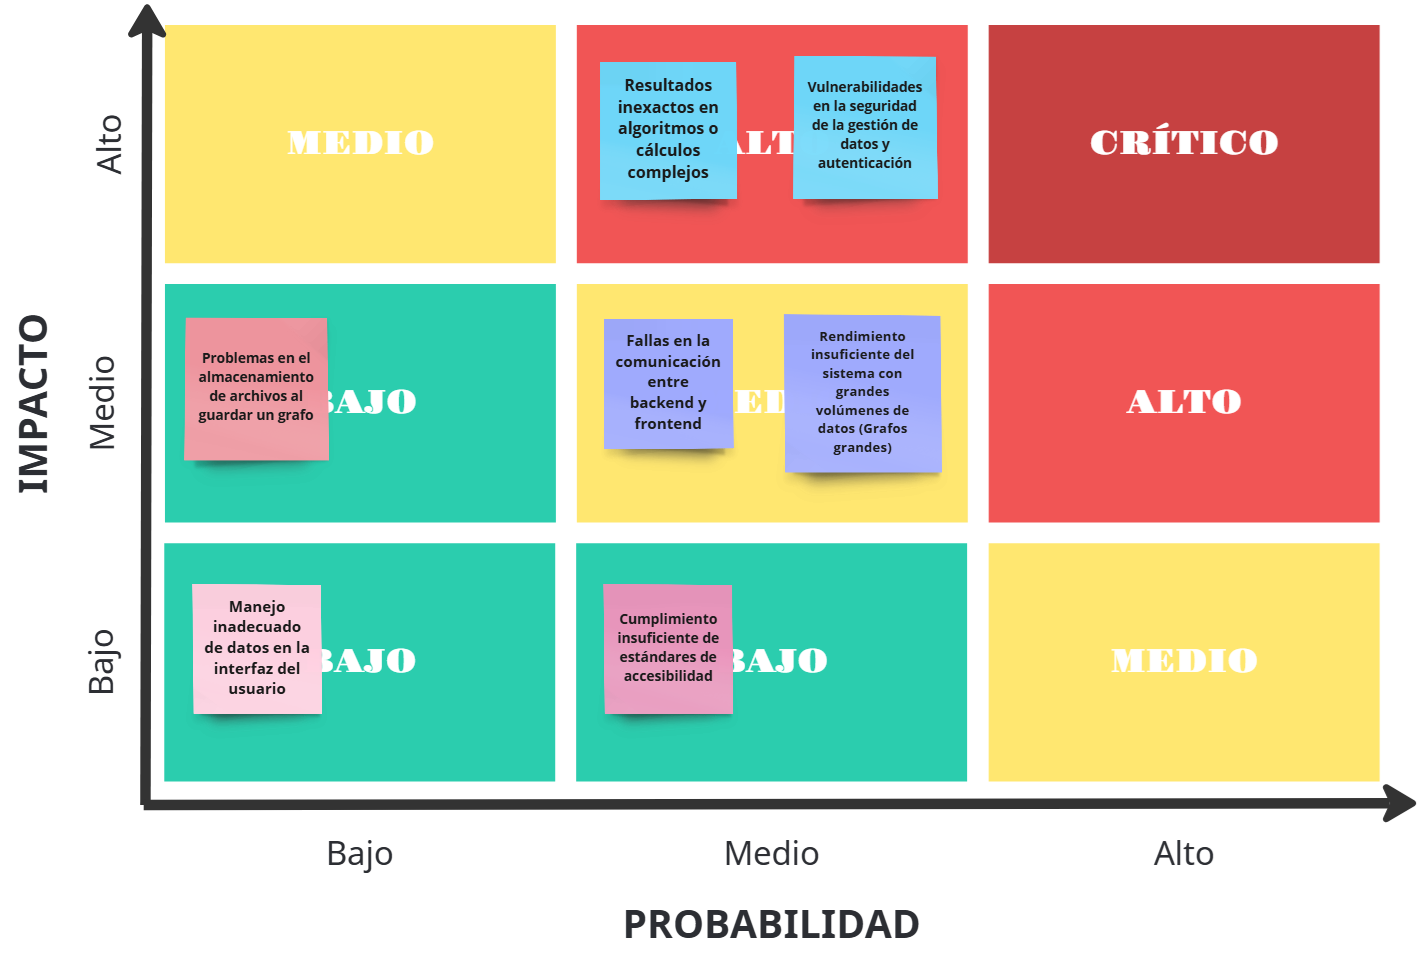
\includegraphics[width=\textwidth]{../imgs/matrix_producto.png}
\end{figure}

\begin{itemize}
    \item \textbf{Resultados inexactos en algoritmos o cálculos complejos} (Probabilidad Media, Impacto Alto): Este riesgo es \textbf{Alto} dado que los cálculos incorrectos pueden comprometer la utilidad y fiabilidad del sistema.
    \item \textbf{Fallas en la comunicación entre backend y frontend} (Probabilidad Media, Impacto Medio): Clasificado como riesgo \textbf{Medio}, aunque podría generar errores visibles para el usuario.
    \item \textbf{Manejo inadecuado de datos en la interfaz del usuario} (Probabilidad Baja, Impacto Bajo): Este riesgo se encuentra en el cuadrante de riesgo \textbf{Bajo} debido a la baja probabilidad de ocurrencia.
    \item \textbf{Rendimiento insuficiente del sistema con grandes volúmenes de datos} (Probabilidad Media, Impacto Medio): Este riesgo está clasificado como \textbf{Medio}, ya que afectaría significativamente el desempeño del sistema.
    \item \textbf{Cumplimiento insuficiente de estándares de accesibilidad} (Probabilidad Media, Impacto Bajo): Clasificado como riesgo \textbf{Bajo}, pero con la posibilidad de afectar la accesibilidad del sistema.
    \item \textbf{Vulnerabilidades en la seguridad de la gestión de datos y autenticación} (Probabilidad Media, Impacto Alto): Este riesgo es \textbf{Alto}, dado que las vulnerabilidades en la seguridad pueden comprometer la integridad del sistema.
    \item \textbf{Problemas en el almacenamiento de archivos al guardar un grafo} (Probabilidad Baja, Impacto Medio): Clasificado como riesgo \textbf{Bajo}, pero puede generar frustración si ocurre.
\end{itemize}

\begin{figure}[H]
    \centering
    \caption{Matriz de Riesgos del Proyecto}
    \label{fig:project_risk_matrix}
    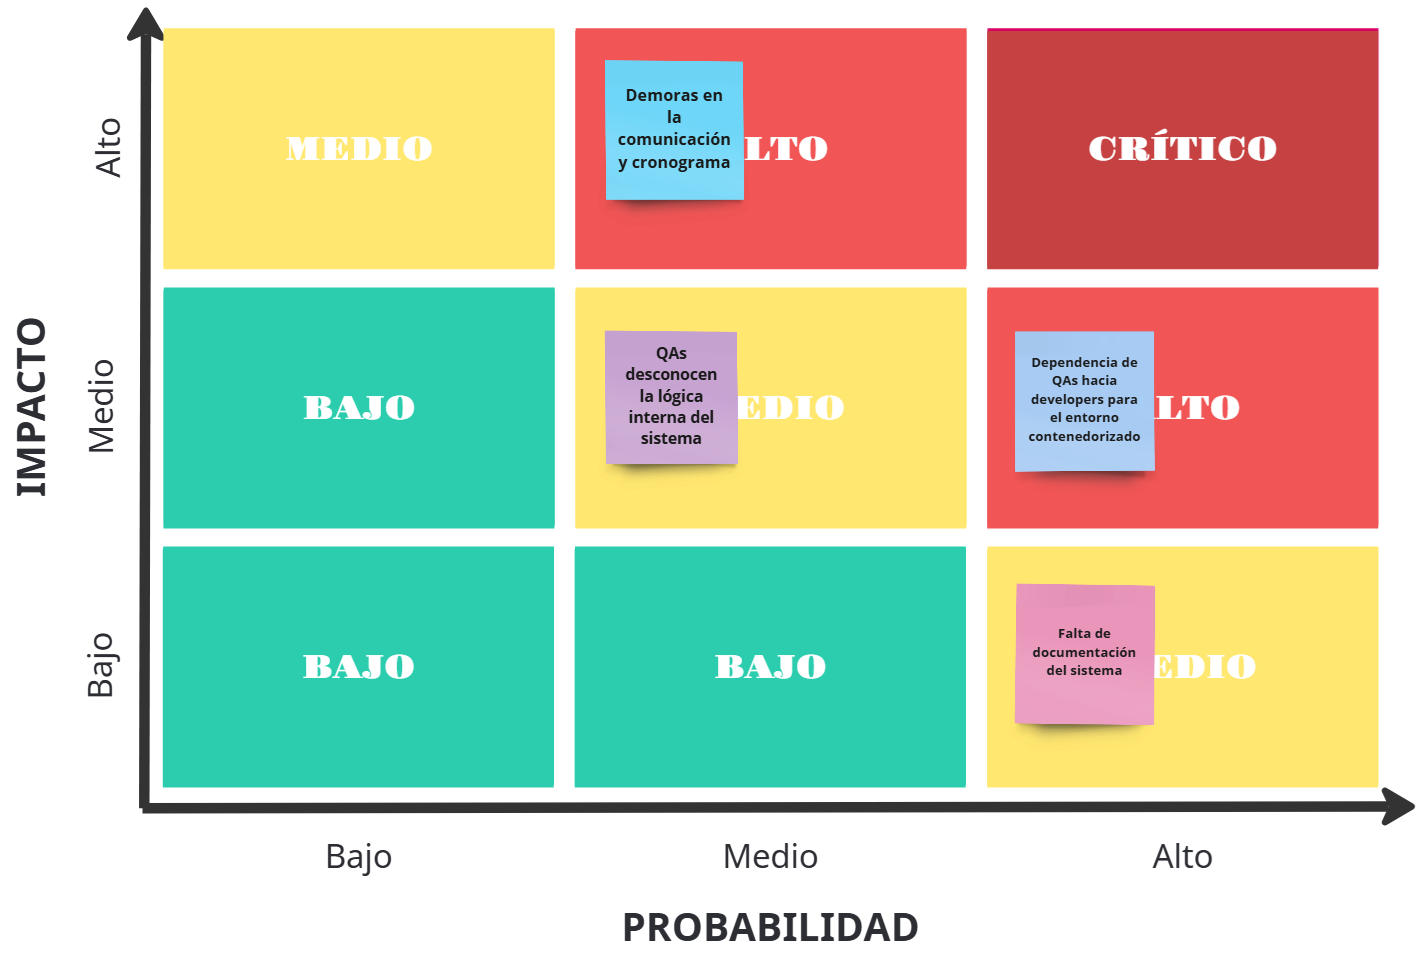
\includegraphics[width=\textwidth]{../imgs/matrix_proyecto.png}
\end{figure}

\begin{itemize}
    \item \textbf{Demoras en la comunicación y cronograma} (Probabilidad Media, Impacto Alto): Este riesgo se encuentra en el cuadrante de riesgo \textbf{Alto}.
    \item \textbf{QAs desconocen la lógica interna del sistema} (Probabilidad Media, Impacto Medio): Clasificado como riesgo \textbf{Medio}, este riesgo necesita medidas de mitigación, como capacitación o documentación adicional.
    \item \textbf{Dependencia de QAs hacia developers para el entorno contenedorizado} (Probabilidad Alta, Impacto Medio): Clasificado como riesgo \textbf{Alto}, este riesgo requiere capacitación y mejora en la gestión de entornos de pruebas.
    \item \textbf{Falta de documentación de los developers} (Probabilidad Alta, Impacto Bajo): Este riesgo se encuentra en el cuadrante de riesgo \textbf{Medio} y necesita controles estrictos para garantizar la disponibilidad de documentación técnica adecuada.
\end{itemize}

\section{\large Presupuesto y Cronograma}

Para el desarrollo del proyecto, se empleó la técnica de estimación de tres puntos, utilizando valores optimistas, pesimistas y los más probables para cada tarea. Este método permitió calcular un rango confiable de tiempo y costo, reduciendo riesgos de sobrecostos o retrasos.

Así se obtuvo:
\begin{itemize}
    \item \textbf{Horas estimadas}: 36 horas para el periodo inicial (1 de diciembre al 15 de diciembre).
\end{itemize}

La estimación final es de \textbf{36 horas-persona} con un \textbf{error estándar aproximado de 4.8 horas-persona}. Esto significa que el esfuerzo estimado es de 36 horas-persona, pero podría variar en un rango de ±4.8 horas debido a posibles incertidumbres. En base a esta estimación, se ha elaborado un cronograma detallado para el proyecto, que se muestra a continuación.

\subsection*{Cronograma del Proyecto}

\begin{table}[H]
    \centering
    \caption{Cronograma del Proyecto}
    \label{fig:cronograma}
    \begin{tabular}{|p{3cm}|p{4cm}|p{4cm}|p{1.8cm}|p{1.8cm}|}
        \hline
        \textbf{Actividad} & \textbf{Descripción} & \textbf{Fecha prevista} & \textbf{Duración (días)} & \textbf{Duración (horas)} \\ \hline
        Organización del Trabajo & Reunión del equipo para definir roles y tareas. & 2024-12-01  & 1 & 2.50 \\ \hline
        Creación del Repositorio & Configuración inicial para pruebas y documentación. & 2024-12-02 & 1 & 1.5 \\ \hline
        Documentación base en LaTeX & Subida de documentos base para el plan y el informe. & 2024-12-02 & 1 & 2.5 \\ \hline
        Pruebas Automatizadas & Realización de pruebas (3 Postman, 3 Playwright). & 2024-12-04 - 2024-12-06 & 3 & 16 \\ \hline
        Documentación Final & Completar y actualizar los documentos en LaTeX. & 2024-12-09 - 2024-12-10 & 2 & 8 \\ \hline
        Revisión y Ajustes Finales & Revisión final de todos los documentos y pruebas. & 2024-12-11 - 2024-12-12 & 2 & 6 \\ \hline
    \end{tabular}
\end{table}

\subsection*{Diagrama Gantt}

\begin{figure}[H]
    \centering
    \caption{Cronograma del Proyecto: Diagrama de Gantt}
    \label{fig:diagrama_gantt}
    \begin{ganttchart}[
        x unit=0.7cm,
        y unit chart=0.7cm,
        hgrid,
        vgrid,
        milestone label font=\scriptsize,
        bar label font=\scriptsize,
        group label font=\scriptsize,
        time slot format=isodate
    ]{2024-12-01}{2024-12-16}
        % Configuración del tiempo
        \gantttitlecalendar{year, month=name, day} \\

        % Actividades
        \ganttbar{Organización del Trabajo}{2024-12-01}{2024-12-01} \\
        \ganttbar{Creación del Repositorio}{2024-12-02}{2024-12-02} \\
        \ganttbar{Documentación base en LaTeX}{2024-12-02}{2024-12-02} \\
        \ganttbar{Pruebas Automatizadas}{2024-12-04}{2024-12-06} \\
        \ganttbar{Documentación Final}{2024-12-09}{2024-12-10} \\
        \ganttbar{Revisión y Ajustes Finales}{2024-12-11}{2024-12-12} \\
        \ganttbar{Entrega del Proyecto}{2024-12-15}{2024-12-15} \\

        % Opcional: Marcar hitos
        \ganttmilestone{Inicio del Proyecto}{2024-12-01} \\
        \ganttmilestone{Fin del Proyecto}{2024-12-15}
    \end{ganttchart}
\end{figure}

El cronograma fue diseñado para ser realista y permitir la realización de las tareas clave del proyecto dentro de un marco temporal adecuado. Las horas estimadas para cada actividad se basaron en la complejidad de las tareas y en la experiencia previa en proyectos similares. Además, se consideraron posibles retrasos o imprevistos, lo que justifica la inclusión del margen de error en la estimación final de horas.

\section{\large Enfoque de Prueba}

\noindent El enfoque de prueba se centra en validar tanto los aspectos funcionales como no funcionales del sistema, asegurando que cumpla con los requisitos definidos y proporcione una experiencia de usuario satisfactoria.

\subsection{Niveles de Prueba}
Para asegurar la calidad del sistema, se realizarán pruebas en los siguientes niveles:
\begin{itemize}
    \item \textbf{Pruebas de Componentes}: Cada funcionalidad clave (como la creación de grafos, generación de matrices, y opciones de optimización) se probará de manera aislada para verificar su correcto funcionamiento.
    \item \textbf{Pruebas de Integración}: Validar la interacción entre componentes, especialmente entre la interfaz y los servicios backend, para asegurar que los datos fluyan correctamente.
    \item \textbf{Pruebas de Sistema}: Se evaluará la funcionalidad del editor, considerando la ejecución fluida de los procesos de prueba, generación de soluciones de optimización, y verificación de resultados.
\end{itemize}

\subsection{Tipos de Prueba}

\noindent En este proyecto, se implementarán diferentes tipos de prueba para asegurar una validación integral del editor \textit{Northwest}, abarcando tanto la funcionalidad como la experiencia de usuario.

\begin{itemize}
    \item \textbf{Pruebas Funcionales}: Estas pruebas aseguran que cada funcionalidad del editor cumpla con los requisitos establecidos, validando que el sistema se comporte como se espera en escenarios específicos. Las pruebas funcionales incluyen:
    \begin{itemize}
        \item \textbf{Validación de Creación y Visualización de Grafos}: Verifica que los grafos se creen correctamente con nodos y conexiones, y se visualicen de manera clara e intuitiva en la interfaz.
        \item \textbf{Carga y Descarga de Archivos}: Asegura que los grafos puedan ser guardados y recuperados sin pérdida de datos ni errores.
        \item \textbf{Generación de Matrices de Adyacencia y Costos}: Comprueba que el editor construya matrices precisas basadas en las conexiones y valores de los nodos.
        \item \textbf{Optimización de Soluciones para diferentes algoritmos}: Valida que el editor produzca soluciones correctas según los distintos algoritmos de optimización seleccionados.
        \item \textbf{Verificación de uso de Interfaz de Usuario (UI)}: Se realizarán pruebas automáticas de la interfaz gráfica para validar la interacción del usuario con el sistema, garantizando la correcta visualización, usabilidad y funcionalidad de los elementos de la interfaz.
        \item \textbf{Verificación de llamadas API}: Se ejecutarán pruebas de los servicios API mediante Postman para garantizar la correcta comunicación entre el cliente y el servidor.
    \end{itemize}

    \item \textbf{Pruebas No Funcionales}: Estas pruebas evalúan los aspectos que afectan la experiencia del usuario, controlando que se cumpla con los criterios de calidad establecidos por la WCAG 2 AA.    
    \begin{itemize}
        \item \textbf{Pruebas de Usabilidad}: Basadas en las heurísticas de Nielsen, estas pruebas aseguran que la interfaz sea intuitiva y satisfactoria para el usuario.
        \item \textbf{Pruebas de Accesibilidad}: Verifican el cumplimiento de estándares básicos de accesibilidad, asegurando que el editor sea utilizable por personas con distintas capacidades.
    \end{itemize}
\end{itemize}



\subsection{Técnicas de Prueba}

\noindent Las técnicas de prueba aplicadas en este proyecto incluyen una combinación de técnicas de caja negra, caja blanca y herramientas específicas para la usabilidad y accesibilidad, para garantizar una validación exhaustiva del editor \textit{Northwest}.

\begin{itemize}
    \item \textbf{Técnicas de Caja Negra}: Se enfocan en la funcionalidad del software sin considerar la estructura interna. Estas pruebas evalúan si el software actúa según lo esperado en diferentes situaciones.
    
    \begin{itemize}
        \item \textbf{Partición de Equivalencias}: Se utilizará para validar que el sistema maneja adecuadamente diferentes categorías de entrada (por ejemplo, valores válidos e inválidos en campos como oferta y demanda), agrupando los datos en clases de equivalencia. Esta técnica permite reducir el número de casos de prueba necesarios al probar solo una entrada representativa por clase.
        \item \textbf{Valores Límite}: Para verificar que los algoritmos respondan correctamente en los extremos de los datos de entrada, asegurando que no ocurran errores con valores cercanos a los límites aceptables.
    \end{itemize}

    \item \textbf{Técnicas para Usabilidad y Accesibilidad}:
    \begin{itemize}
        \item \textbf{Pruebas Basadas en Listas de Verificación (Checklists)}: Enfocadas en usabilidad, estas pruebas se basarán en listas de verificación construidas a partir de heurísticas de usabilidad de Nielsen para evaluar la facilidad de uso de la interfaz. La lista incluirá aspectos como claridad de la interfaz, accesibilidad de los elementos y consistencia en el diseño.
        \item \textbf{Pruebas de Accesibilidad con Axe DevTools}: Para verificar el cumplimiento de criterios de accesibilidad, se empleará la herramienta Axe DevTools, que permite realizar pruebas automáticas de accesibilidad en la interfaz y detectar posibles problemas, como bajo contraste de colores, falta de etiquetas en elementos interactivos y problemas de navegabilidad. Los resultados obtenidos con Axe DevTools se documentarán en el reporte de accesibilidad, asegurando que el sistema cumpla con estándares de accesibilidad propuestos por la WCAG 2 AA.
    \end{itemize}
\end{itemize}


\subsection{Criterios de Entrada y Salida}
\begin{itemize}
    \item \textbf{Criterios de Entrada}: Para iniciar la fase de pruebas, deben cumplirse las siguientes condiciones:
    \begin{itemize}
        \item Todos los servicios de backend estén configurados y ejecutándose en Docker.
        \item El entorno de frontend esté disponible, ya sea ejecutándose en Docker o localmente.
        \item La interfaz de usuario y los servicios backend estén disponibles y comunicándose correctamente.
        \item Todos los requisitos de datos de prueba estén definidos, incluyendo configuraciones específicas para nodos, matrices y otros parámetros requeridos.
        \item Acceso a las historias de usuario para revisar requisitos y objetivos específicos de cada funcionalidad.
        \item Se tienen habilitadas las herramientas necesarias para realizar las pruebas, como: Postman, herramientas de accesibilidad y de pruebas de interfaz.
    \end{itemize}
    
    \item \textbf{Criterios de Salida}: Las pruebas se considerarán finalizadas cuando:
    \begin{itemize}
        \item Se hayan ejecutado en su totalidad los casos de prueba propuestos y se hayan documentado sus resultados y observaciones.
        \item Se haya finalizado el análisis de defectos encontrados y todos los hallazgos estén documentados en el informe de resultados.
        \item Todos los criterios de éxito para alcanzar el nivel \texttt{AA} en la normativa WCAG de accesibilidad hayan sido evaluados y cumplidos.
        \item Se haya completado el checklist de usabilidad basado en las heurísticas de Nielsen, asegurando una experiencia de usuario óptima.
        \item Todas las métricas definidas se hayan recopilado para el análisis de resultados.
    \end{itemize}
\end{itemize}

\subsection{Independencia de las Pruebas}
Dado que parte del equipo de desarrollo participa también en el proceso de pruebas, las pruebas no serán completamente independientes. Para mitigar posibles conflictos de interés, se establecerán procedimientos claros para la documentación y revisión de resultados, asegurando que las pruebas sean objetivas y confiables.

\subsection{Métricas a Ser Recopiladas}
Para evaluar la efectividad y calidad de las pruebas, se recopilarán las siguientes métricas, incluyendo aquellas derivadas del análisis de resultados:

\begin{itemize}
    \item \textbf{Tasa de éxito de Test Cases}: Porcentaje de pruebas exitosas sobre el total de casos ejecutados.
    \item \textbf{Cobertura de requisitos del usuario}: Porcentaje de historias de usuario cubiertas por pruebas realizadas.
    \item \textbf{Número y tipo de defectos identificados}: Total de defectos encontrados, categorizados según funcionalidad, usabilidad y accesibilidad.
    \item \textbf{Defectos resueltos vs. pendientes}: Proporción de defectos corregidos en relación con los detectados.
    \item \textbf{Tiempo total de ejecución de pruebas}: Tiempo en horas-persona requerido para completar las pruebas.
    \item \textbf{Automatización de Test Cases}: Resultados de pruebas automatizadas, diferenciando las herramientas utilizadas y los resultados obtenidos.
    \item \textbf{Tiempo Medio de Reparación (TMR)}: Tiempo promedio requerido para corregir defectos críticos, desde su detección hasta su resolución.
    \item \textbf{Impacto de accesibilidad}: Alertas detectadas y corregidas en análisis realizados con herramientas como \textit{Axe Dev Tools}.
\end{itemize}


\subsection{Requisitos de Datos de Prueba}
Para llevar a cabo las pruebas, los datos de prueba deben incluir:
\begin{itemize}
    \item Incluir diversas configuraciones de tamaño y complejidad de los grafos para abarcar un amplio espectro de escenarios.
    \item Incluir casos con restricciones específicas para evaluar la robustez y flexibilidad de los algoritmos.
    \item Los arcos deben contener valores que cubran rangos amplios, incluyendo pesos negativos, valores extremos y valores cercanos a los límites aceptables, para simular distintas situaciones de uso.
    \item Se deben incluir datos de entrada no válidos para probar la capacidad de los algoritmos de manejar errores de forma controlada y sin interrupciones.
\end{itemize}

\subsection{Requisitos del Entorno de Prueba}
Los servicios necesarios en el entorno de prueba incluyen:

\begin{itemize}
    \item \textbf{Backend implementado en FastAPI}: Este servicio maneja las solicitudes de optimización de transporte y debe estar configurado para responder a peticiones de la interfaz y los cálculos de matrices, asegurando un procesamiento eficiente y consistente de datos.
    \item \textbf{Servicios de almacenamiento}: Configurados para gestionar y almacenar archivos de configuración en formato JSON. Estos servicios garantizan la persistencia de datos y permiten la carga y recuperación de grafos y matrices sin pérdida de información.
    \item \textbf{Frontend desarrollado en Vue.js}: La interfaz gráfica del editor, desarrollada en Vue.js, permite la interacción del usuario con los elementos del editor. El frontend puede ejecutarse en Docker o de manera local, asegurando accesibilidad a todas las funcionalidades requeridas para la prueba.
    \item \textbf{Buscador web}: Disponibilidad de un buscador de donde pueda realizarse el acceso al sistema.
    \item \textbf{Herramientas de prueba}: Estas herramientas (tales como Postman, Axe DevTools y Playwright) deben estar activas para la ejecución de los test cases.

\end{itemize}

Además, para asegurar la integridad del entorno, todos los servicios deben estar conectados mediante una red interna en Docker, permitiendo una comunicación fluida entre los contenedores. Esta configuración facilitará la ejecución de pruebas automáticas y manuales en un entorno controlado, simulado y con condiciones similares a las de producción.

\subsection{Desviación de la Política de pruebas y estrategia de pruebas de la empresa}
Este plan de pruebas sigue los lineamientos establecidos por la política y estrategia de pruebas de los propietarios del software, cumpliendo con los estándares de calidad y verificación esperados.
\newpage
% Referencias
\renewcommand\refname{\large\textbf{Referencias}}
\bibliographystyle{apacite}
\bibliography{mibibliografia}
\cite{nielsen1994}
\cite{dennis2015}
\cite{gregory2023}

\clearpage
\section{\large Anexos}
\subsection{Anexo A: Historias de Usuario}
\begin{table}[!ht]
    \centering
    \caption{Historia de Usuario HU001-SignUp/SignIn-01}
    \label{tab:HU001-SignUp/SignIn-01}
    \userstory{HU001-SignUp/SignIn-01}{usuario nuevo}{poder registrarme proporcionando mi correo electrónico, nombre de usuario y contraseña,}{crear una cuenta y acceder a la aplicación.}{https://github.com/go-to-hell/proyecto-grafos-front/issues/82}
\end{table}

\begin{table}[!ht]
    \centering
    \caption{Historia de Usuario HU002-SignUp/SignIn-02}
    \label{tab:HU002-SignUp/SignIn-02}
    \userstory{HU002-SignUp/SignIn-02}{usuario que se está registrando}{recibir mensajes de error claros si introduzco un correo electrónico inválido o una contraseña débil,}{saber qué debo corregir antes de completar mi registro.}{https://github.com/go-to-hell/proyecto-grafos-front/issues/83}
\end{table}

\begin{table}[!ht]
    \centering
    \caption{Historia de Usuario HU003-SignUp/SignIn-03}
    \label{tab:HU003-SignUp/SignIn-03}
    \userstory{HU003-SignUp/SignIn-03}{usuario registrado}{ingresar mi correo electrónico y contraseña en una pantalla de inicio de sesión,}{acceder a mi cuenta y a las funcionalidades de la aplicación.}{https://github.com/go-to-hell/proyecto-grafos-front/issues/84}
\end{table}

\begin{table}[!ht]
    \centering
    \caption{Historia de Usuario HU004-Johnson-01}
    \label{tab:HU004-Johnson-01}
    \userstory{HU004-Johnson-01}{usuario}{construir una representación de un problema de ruta crítica (CPM) como un grafo con actividades en las aristas,}{identificar la ruta crítica utilizando el algoritmo de Johnson.}{https://github.com/go-to-hell/proyecto-grafos-front/issues/48}
\end{table}

\begin{table}[!ht]
    \centering
    \caption{Historia de Usuario HU005-Johnson-02}
    \label{tab:HU005-Johnson-02}
    \userstory{HU005-Johnson-02}{usuario}{descargar un grafo como archivo local,}{poder continuarlo más tarde.}{https://github.com/go-to-hell/proyecto-grafos-front/issues/49}
\end{table}

\begin{table}[!ht]
    \centering
    \caption{Historia de Usuario HU006-GraphEditor-01}
    \label{tab:HU006-GraphEditor-01}
    \userstory{HU006-GraphEditor-01}{usuario de la aplicación}{poder agregar nodos, aristas y editar sus valores,}{poder construir y modificar gráficos de manera interactiva y visual.}{https://github.com/go-to-hell/proyecto-grafos-front/issues/50}
\end{table}

\begin{table}[!ht]
    \centering
    \caption{Historia de Usuario HU007-AdjacentMatrix-01}
    \label{tab:HU007-AdjacentMatrix-01}
    \userstory{HU007-AdjacentMatrix-01}{usuario de la aplicación}{obtener la matriz de adyacencia del grafo generado,}{poder visualizar las conexiones entre los nodos de forma estructurada y utilizar esta información posteriormente.}{https://github.com/go-to-hell/proyecto-grafos-front/issues/51}
\end{table}

\begin{table}[!ht]
    \centering
    \caption{Historia de Usuario HU008-FileManagement-01}
    \label{tab:HU008-FileManagement-01}
    \userstory{HU008-FileManagement-01}{usuario de la aplicación}{poder guardar el grafo realizado en formato JSON,}{cargarlo posteriormente y abrirlo en el mismo estado en el que lo dejé, conservando todos los nodos, aristas y configuraciones.}{https://github.com/go-to-hell/proyecto-grafos-front/issues/52}
\end{table}

\begin{table}[!ht]
    \centering
    \caption{Historia de Usuario HU009-NorthWest-01}
    \label{tab:HU009-NorthWest-01}
    \userstory{HU009-NorthWest-01}{usuario del sistema}{que la matriz de costos se genere automáticamente al crear nodos y conexiones,}{asegurarme de que los valores de los pesos reflejan correctamente las relaciones entre puntos de suministro y demanda.}{https://github.com/go-to-hell/proyecto-grafos-front/issues/53}
\end{table}

\begin{table}[!ht]
    \centering
    \caption{Historia de Usuario HU010-NorthWest-02}
    \label{tab:HU010-NorthWest-02}
    \userstory{HU010-NorthWest-02}{usuario del sistema}{manejar desequilibrios entre oferta y demanda, validando los campos obligatorios en el formulario de entrada,}{asegurarme de que se ajusten las soluciones automáticamente, evitando errores en el cálculo del transporte, y que pueda ingresar mis datos sin problemas, recibiendo retroalimentación clara en caso de errores.}{https://github.com/go-to-hell/proyecto-grafos-front/issues/54}
\end{table}

\begin{table}[!ht]
    \centering
    \caption{Historia de Usuario HU011-NorthWest-03}
    \label{tab:HU011-NorthWest-03}
    \userstory{HU011-NorthWest-03}{usuario del sistema}{generar soluciones válidas para las diferentes configuraciones que me da el sistema,}{poder confiar en la validez de los resultados y obtener diferentes resultados basados en el criterio de optimización que elija.}{https://github.com/go-to-hell/proyecto-grafos-front/issues/55}
\end{table}

\begin{table}[!ht]
    \centering
    \caption{Historia de Usuario HU012-Kruskal-01}
    \label{tab:HU012-Kruskal-01}
    \userstory{HU012-Kruskal-01}{usuario de la aplicación}{poder aplicar el algoritmo de Kruskal en el editor de grafos para encontrar el árbol de expansión mínimo o máximo,}{visualizar y analizar la ruta óptima entre los nodos seleccionados y obtener el valor total de la suma de los pesos de dicha ruta.}{https://github.com/go-to-hell/proyecto-grafos-front/issues/57}
\end{table}

\begin{table}[!ht]
    \centering
    \caption{Historia de Usuario HU013-Dijkstra-01}
    \label{tab:HU013-Dijkstra-01}
    \userstory{HU013-Dijkstra-01}{usuario del sistema}{que el algoritmo de Dijkstra me devuelva el camino más corto en el grafo con la menor cantidad de recursos posibles,}{visualizar y analizar la ruta óptima entre los nodos seleccionados y obtener el valor total de la suma de los pesos de dicha ruta.}{https://github.com/go-to-hell/proyecto-grafos-front/issues/58}
\end{table}

\begin{table}[!ht]
    \centering
    \caption{Historia de Usuario HU014-InvalidData-01}
    \label{tab:HU014-InvalidData-01}
    \userstory{HU014-InvalidData-01}{usuario administrador del sistema}{que el sistema valide y maneje los datos no válidos que se ingresan en los algoritmos,}{poder corregir los errores rápidamente y que el sistema no presente fallos graves.}{https://github.com/go-to-hell/proyecto-grafos-front/issues/59}
\end{table}

\begin{table}[!ht]
    \centering
    \caption{Historia de Usuario HU015-Dashboard-01}
    \label{tab:HU015-Dashboard-01}
    \userstory{HU015-Dashboard-01}{usuario del sistema}{que la interfaz del dashboard se actualice al modificar los nodos o arcos en el grafo,}{poder ver reflejados mis cambios inmediatamente y asegurarme de que el algoritmo calcule con los datos actualizados.}{https://github.com/go-to-hell/proyecto-grafos-front/issues/60}
\end{table}

\begin{table}[!ht]
    \centering
    \caption{Historia de Usuario HU016-AccesibilityAndNavigation-01}
    \label{tab:HU016-AccesibilityAndNavigation-01}
    \userstory{HU016-AccesibilityAndNavigation-01}{usuario con discapacidades}{que el sistema sea accesible y que el contraste de los elementos de la interfaz cumpla con estándares de accesibilidad,}{poder utilizar el sistema sin barreras visuales y facilitar mi interacción.}{https://github.com/go-to-hell/proyecto-grafos-front/issues/61}
\end{table}

\begin{table}[!ht]
    \centering
    \caption{Historia de Usuario HU017-Compet-01}
    \label{tab:HU017-Compet-01}
    \userstory{HU017-Compet-01}{usuario del sistema}{que el algoritmo de Compet procese grafos que incluyen nodos y arcos con valores extremos y negativos,}{poder verificar rutas que consideren correctamente estos valores y obtener soluciones precisas y optimizadas.}{https://github.com/go-to-hell/proyecto-grafos-front/issues/62}
\end{table}

\begin{table}[!ht]
    \centering
    \caption{Historia de Usuario HU018-AccesibilityAndNavigation-02}
    \label{tab:HU018-AccesibilityAndNavigation-02}
    \userstory{HU018-AccesibilityAndNavigation-02}{usuario del sistema}{que cada algoritmo cuente con textos de ayuda o "helps" que expliquen su función y pasos de uso,}{poder comprender cómo funciona cada algoritmo y cómo utilizarlo correctamente en el sistema.}{https://github.com/go-to-hell/proyecto-grafos-front/issues/63}
\end{table}

\begin{table}[!ht]
    \centering
    \caption{Historia de Usuario HU019-Sorts-01}
    \label{tab:HU019-Sorts-01}
    \userstory{HU019-Sorts-01}{usuario que quiere ordenar datos}{ingresar una lista de números (o cargar un archivo),}{que el sistema los ordene usando diferentes algoritmos de ordenamiento disponibles.}{https://github.com/go-to-hell/proyecto-grafos-front/issues/64}
\end{table}

\begin{table}[!ht]
    \centering
    \caption{Historia de Usuario HU020-Sorts-02}
    \label{tab:HU020-Sorts-02}
    \userstory{HU020-Sorts-02}{usuario que está probando el módulo de ordenamiento}{poder elegir entre varios algoritmos de ordenamiento (Selection Sort, Insertion Sort, Merge Sort, Shell Sort),}{observar y entender cómo funciona cada método visualmente.}{https://github.com/go-to-hell/proyecto-grafos-front/issues/65}
\end{table}

\begin{table}[!ht]
    \centering
    \caption{Historia de Usuario HU021-Sorts-03}
    \label{tab:HU021-Sorts-03}
    \userstory{HU021-Sorts-03}{usuario interesado en el módulo de ordenamiento}{ver una animación paso a paso que me muestre cómo se ordenan los elementos,}{aprender cómo el algoritmo organiza los datos.}{https://github.com/go-to-hell/proyecto-grafos-front/issues/66}
\end{table}

\begin{table}[!ht]
    \centering
    \caption{Historia de Usuario HU022-Sorts-04}
    \label{tab:HU022-Sorts-04}
    \userstory{HU022-Sorts-04}{usuario que observa la visualización del ordenamiento}{ajustar la velocidad de la animación,}{adaptar el ritmo de la visualización a mis necesidades.}{https://github.com/go-to-hell/proyecto-grafos-front/issues/67}
\end{table}

\begin{table}[!ht]
    \centering
    \caption{Historia de Usuario HU023-Sorts-05}
    \label{tab:HU023-Sorts-05}
    \userstory{HU023-Sorts-05}{usuario que desea probar los algoritmos de ordenamiento con diferentes conjuntos de datos}{generar automáticamente una lista de números aleatorios en el módulo de Sorts,}{poder ordenar fácilmente un conjunto de datos sin tener que ingresarlos.}{https://github.com/go-to-hell/proyecto-grafos-front/issues/68}
\end{table}

\begin{table}[!ht]
    \centering
    \caption{Historia de Usuario HU024-BinaryTrees-01}
    \label{tab:HU024-BinaryTrees-01}
    \userstory{HU024-BinaryTrees-01}{usuario que trabaja con datos específicos}{poder guardar un arreglo y cargarlo en el módulo,}{reutilizar datos sin tener que ingresarlos manualmente cada vez.}{https://github.com/go-to-hell/proyecto-grafos-front/issues/69}
\end{table}

\begin{table}[!ht]
    \centering
    \caption{Historia de Usuario HU025-BinaryTrees-02}
    \label{tab:HU025-BinaryTrees-02}
    \userstory{HU025-BinaryTrees-02}{usuario que quiere trabajar con estructuras de datos}{ingresar valores para construir un árbol binario visual,}{entender y ver la estructura resultante.}{https://github.com/go-to-hell/proyecto-grafos-front/issues/70}
\end{table}

\begin{table}[!ht]
    \centering
    \caption{Historia de Usuario HU026-BinaryTrees-03}
    \label{tab:HU026-BinaryTrees-03}
    \userstory{HU026-BinaryTrees-03}{usuario que estudia los árboles binarios}{ver los recorridos del árbol (preorden, inorden, postorden),}{entender cómo funcionan las diferentes formas de recorrer un árbol binario.}{https://github.com/go-to-hell/proyecto-grafos-front/issues/71}
\end{table}

\begin{table}[!ht]
    \centering
    \caption{Historia de Usuario HU027-BinaryTrees-04}
    \label{tab:HU027-BinaryTrees-04}
    \userstory{HU027-BinaryTrees-04}{usuario que interactúa con árboles binarios}{poder ingresar valores para construir el árbol,}{visualizar y analizar la estructura resultante sin la necesidad de editar o eliminar nodos.}{https://github.com/go-to-hell/proyecto-grafos-front/issues/72}
\end{table}

\begin{table}[!ht]
    \centering
    \caption{Historia de Usuario HU028-BinaryTrees-05}
    \label{tab:HU028-BinaryTrees-05}
    \userstory{HU028-BinaryTrees-05}{usuario que quiere explorar la estructura completa del árbol}{centrar y ajustar el gráfico,}{ver el árbol completo de forma clara sin tener que desplazarme mucho.}{https://github.com/go-to-hell/proyecto-grafos-front/issues/73}
\end{table}

\begin{table}[!ht]
    \centering
    \caption{Historia de Usuario HU029-BinaryTrees-06}
    \label{tab:HU029-BinaryTrees-06}
    \userstory{HU029-BinaryTrees-06}{usuario que quiere preservar su trabajo}{guardar la estructura del árbol binario y cargarla en futuras sesiones,}{continuar trabajando en el árbol o analizarlo en otro momento.}{https://github.com/go-to-hell/proyecto-grafos-front/issues/74}
\end{table}

\begin{table}[!ht]
    \centering
    \caption{Historia de Usuario HU030-Asignation-01}
    \label{tab:HU030-Asignation-01}
    \userstory{HU030-Asignation-01}{usuario}{tener una opción,}{resolver la asignación.}{https://github.com/go-to-hell/proyecto-grafos-front/issues/78}
\end{table}

\begin{table}[!ht]
    \centering
    \caption{Historia de Usuario HU031-Asignation-02}
    \label{tab:HU031-Asignation-02}
    \userstory{HU031-Asignation-02}{usuario}{visualizar el resultado de la asignación,}{recibir una respuesta.}{https://github.com/go-to-hell/proyecto-grafos-front/issues/79}
\end{table}

\begin{table}[!ht]
    \centering
    \caption{Historia de Usuario HU032-Asignation-03}
    \label{tab:HU032-Asignation-03}
    \userstory{HU032-Asignation-03}{usuario}{elegir entre Maximizar o Minimizar la Asignación,}{recibir una respuesta acorde a mis necesidades.}{https://github.com/go-to-hell/proyecto-grafos-front/issues/80}
\end{table}

\begin{table}[!ht]
    \centering
    \caption{Historia de Usuario HU033-Asignation-04}
    \label{tab:HU033-Asignation-04}
    \userstory{HU033-Asignation-04}{usuario}{tener la opción del Algoritmo de Asignación,}{poder usarlo.}{https://github.com/go-to-hell/proyecto-grafos-front/issues/81}
\end{table}

\clearpage
\subsection{Anexo B: Diagramas de Flujo y Arquitectura}    
\begin{figure}[H]
    \centering
    \label{fig:architecture}
    \caption{Arquitectura del sistema y sus interacciones principales}
    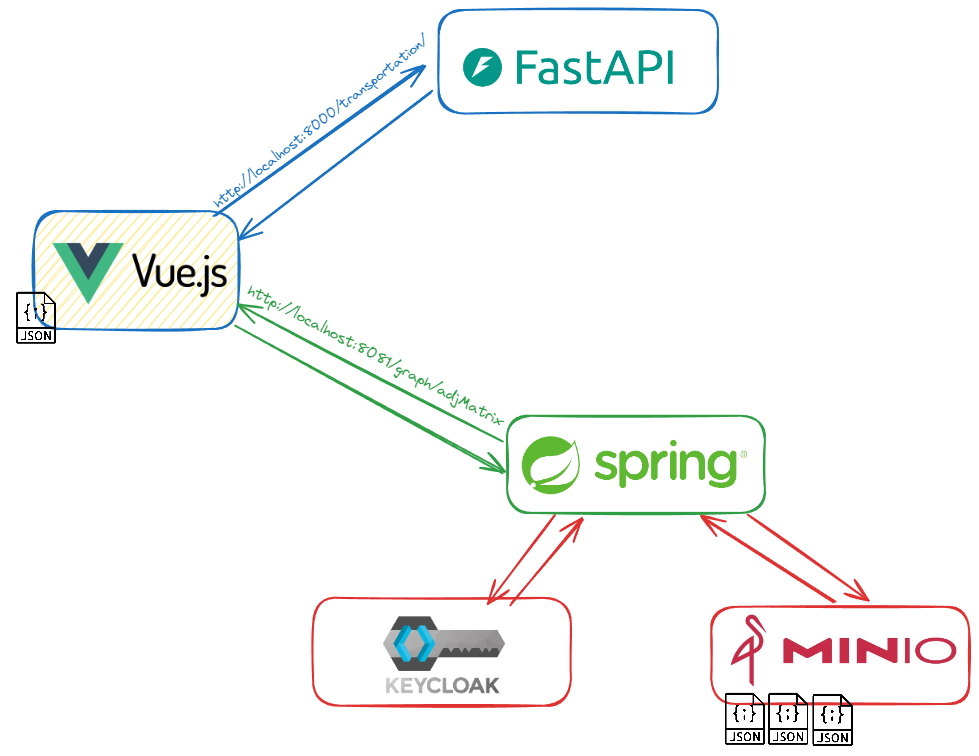
\includegraphics[width=\textwidth]{../imgs/architecture-2024-03-18-2220.png}
\end{figure}

\clearpage
\subsection{Anexo C: Plantilla de Reporte de Defectos}

\begin{longtable}{|p{5cm}|p{10cm}|}
    \caption{Plantilla de Reporte de Defectos} \label{tab:reporte_defectos} \\
    \hline
    \textbf{Código} & \\ \hline
    \textbf{Descripción} & \\ \hline
    \textbf{Pasos para reproducir} & 
    1. \newline
    2. \newline
    3. \\ \hline
    \textbf{Resultado esperado} & \\ \hline
    \textbf{Resultado actual} & \\ \hline
    \textbf{Severidad} & \\ \hline
    \textbf{Evidencia} & \\ \hline
    \textbf{Fecha detección} & \\ \hline
    \textbf{Fecha resolución} & \\ \hline
    \textbf{TMR} & \\ \hline
    \textbf{Estado ejecución} & \\ \hline
\end{longtable}

\subsection{Anexo D: Plantilla de Casos de Prueba}

\begin{longtable}{|p{5cm}|p{10cm}|}
    \caption{Plantilla de Casos de Prueba} \label{tab:plantilla_caso_prueba} \\
    \hline
    \textbf{Código} & \\ \hline
    \textbf{Descripción} & \\ \hline
    \textbf{Pre condiciones} & \\ \hline
    \textbf{Pasos para reproducir} & 
    1. \newline
    2. \newline
    3. \\ \hline
    \textbf{Resultado esperado}  & 
    1. \newline
    2. \newline
    3. \\ \hline
    \textbf{Severidad} & \\ \hline
    \textbf{Evidencias} & \\ \hline
    \textbf{Documentación} & \\ \hline
    \textbf{Estado ejecución} & \\ \hline
\end{longtable}


\addcontentsline{toc}{subsection}{Anexo E: Pruebas Planificadas}

% Define the section but make it invisible

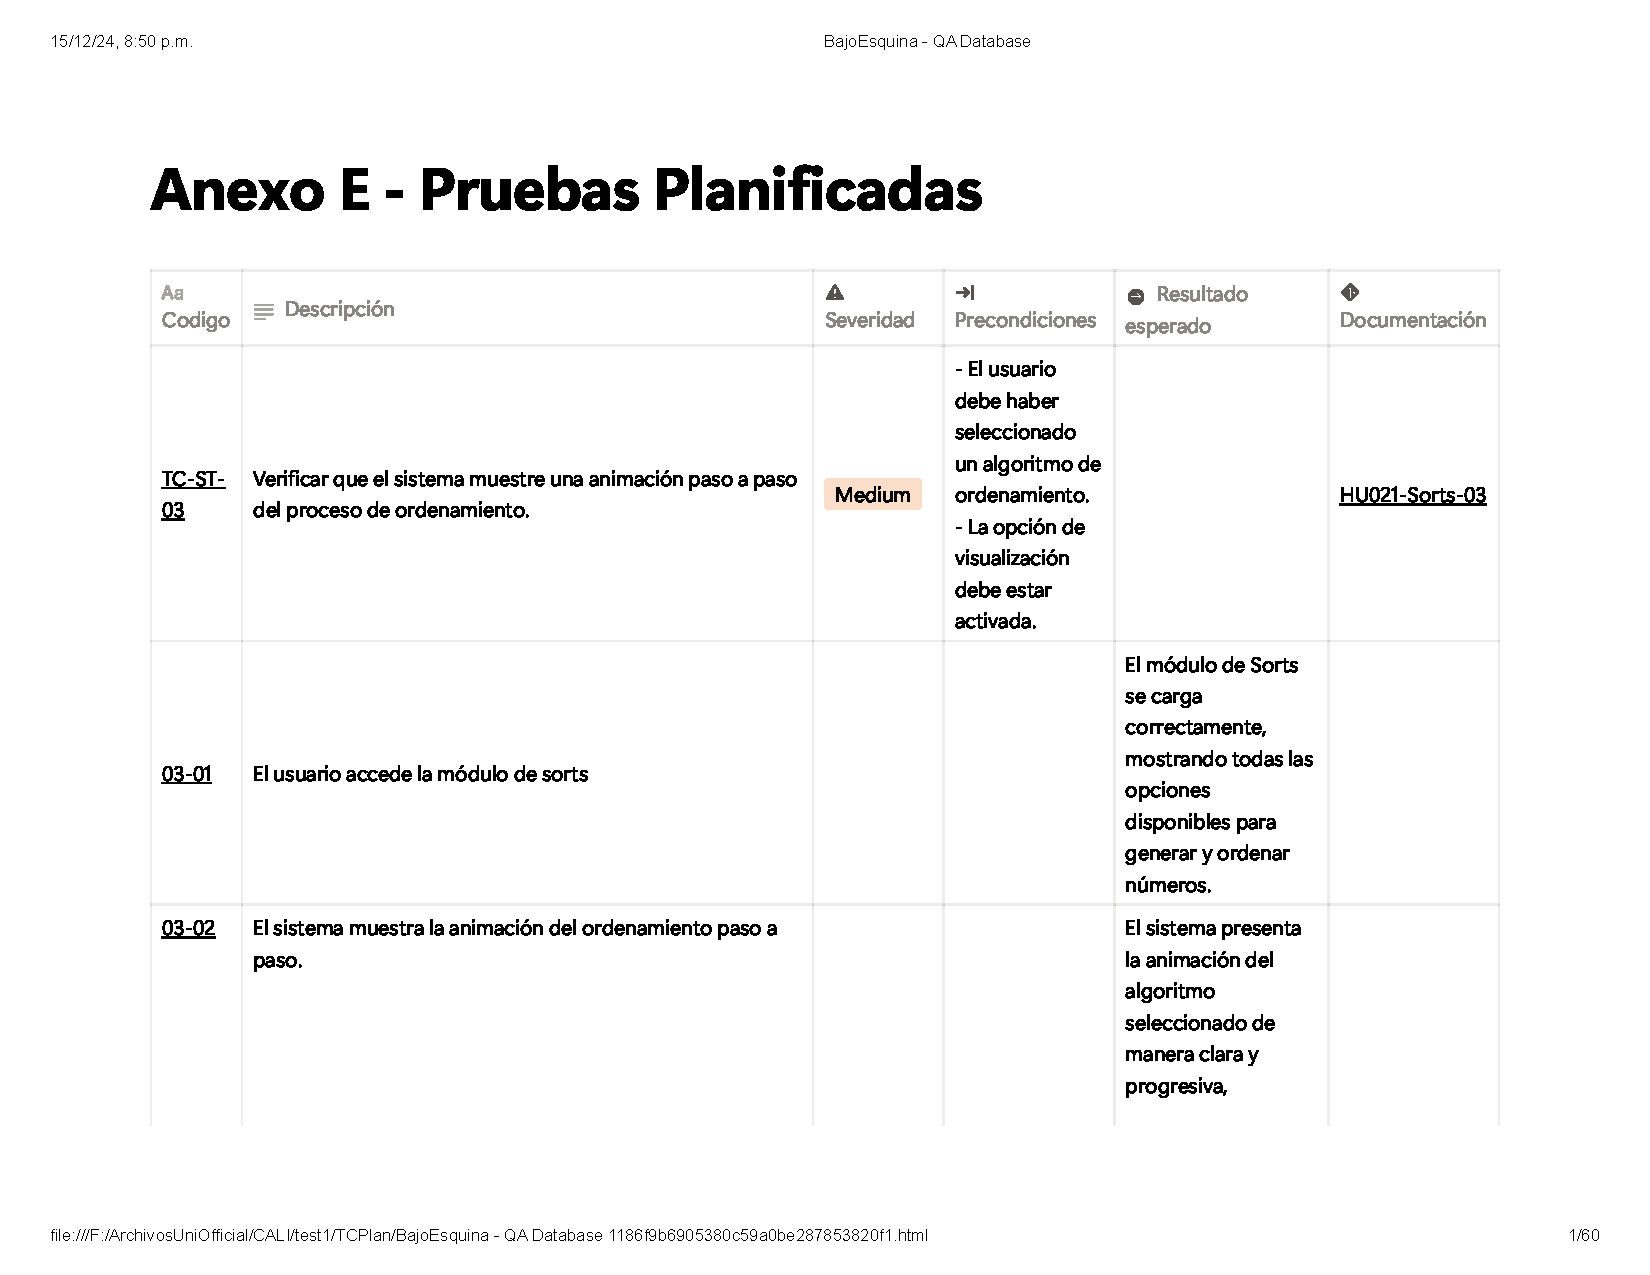
\includepdf[pages=-]{plannedtests.pdf}
\phantomsection
\subsection{Anexo F: Plantilla de Historias de Usuario}

\begin{table}[!ht]
    \centering
    \caption{Historia de Usuario HU001-Codigo-01}
    \label{tab:plantilla_historia_usuario}
    \userstory{HU001-Codigo-01}{usuario}{...,}{...}{https://github.com/go-to-hell/proyecto-grafos-front/issues/81}
\end{table}

\subsection{Anexo G: Plantilla de Reporte de Usabilidad}
\begin{longtable}{|>{\raggedright\arraybackslash}p{10cm}|>{\centering\arraybackslash}p{3cm}|}
    \caption{Plantilla de Reporte de Usabilidad} \label{tab:reporte_usabilidad} \\
    \hline
    \textbf{Items} & \textbf{Evaluation} \\ \hline
    
    \textbf{1.- Visibilidad del estado del sistema} & \\ \hline
    ¿Cada parte de la interfaz comienza con un título que describa el contenido de la pantalla? & \\ \hline
    ¿El diseño de íconos y su estética es consistente en todo el sistema? & \\ \hline
    Cuando se selecciona un icono que está rodeado de otros iconos, ¿Se distingue claramente el ícono seleccionado? & \\ \hline
    Si se utilizan ventanas emergentes (pop-up) para mostrar mensajes de error, ¿Permiten esas ventanas que el usuario visualice el error en la interfaz cuando se despliegan? & \\ \hline
    ¿Hay algún tipo de feedback para cada acción u operación? & \\ \hline
    Luego de que el usuario completa una acción o serie de acciones, ¿El "feedback" del sistema indica que el siguiente grupo de acciones puede completarse? & \\ \hline
    El sistema provee algún tipo de feedback visual en menús o cajas de diálogo que indiquen qué opciones pueden seleccionarse. & \\ \hline
    El sistema provee algún tipo de feedback visual en menús o cajas de diálogo que indiquen en cuál de las posibles opciones se halla posicionado el cursor. & \\ \hline
    Si hay menús o caja de diálogo en donde pueden seleccionarse múltiples opciones, ¿El sistema provee algún tipo de "feedback" visual que indique cuáles son las opciones ya seleccionadas? & \\ \hline
    ¿El sitio web entrega información corporativa de la organización? & \\ \hline
    Si existen demoras mayores a 15 segundos en las respuestas del sistema, ¿El usuario es informado del progreso en la concreción de la respuesta? & \\ \hline
    ¿Informa datos relevantes para quien no "navega" (Ej: Horas de atención)? ¿Y para hacer consultas web o no web (Ej: números de teléfono)? & \\ \hline
    ¿Los tiempos de respuesta son apropiados para cada tarea? & \\ \hline
    Tiempo de escritura, movimiento del cursor o selección con el ratón: entre 0,5 y 1,5 milisegundos & \\ \hline
    Tareas más comunes: 2 a 4 segundos & \\ \hline
    Tareas complejas: 8 a 12 segundos & \\ \hline
    No son necesarios altos niveles de concentración y no es requerido retener información: 2 a 15 segundos & \\ \hline
    La terminología usada en los menús, ¿Es consistente con el dominio de conocimiento del usuario en relación a la tarea a realizar? & \\ \hline
    ¿El usuario conoce su ruta de ubicación? & \\ \hline
    
    \textbf{2.- Relación entre el sistema y el mundo real} & \\ \hline
    ¿Los íconos son concretos y familiares para el usuario? & \\ \hline
    ¿Los colores seleccionados corresponden a los valores esperados? & \\ \hline
    Cuando se ingresan datos en la pantalla, ¿La terminología utilizada para describir la tarea es familiar para los usuarios? & \\ \hline
    Cuando la pantalla incluye preguntas, ¿El lenguaje de esas preguntas es claro y conciso? & \\ \hline
    Las combinaciones de secuencias de letras o palabras extrañas o poco frecuentes, ¿Se evitan siempre que sea posible? & \\ \hline
    El sistema ingresa/elimina de manera automática los signos de pesos o dólar y decimal cuando se insertan valores monetarios. & \\ \hline
    ¿Se utilizan nombres unívocos y descriptivos en todo momento? & \\ \hline
    ¿Se hace uso de los rastreadores de progreso? & \\ \hline
    Los H1 están optimizados para SEO & \\ \hline
    
    \textbf{3.- Control y libertad  por parte del usuario} & \\ \hline
    En sistemas que permitan el uso de ventanas superpuestas ¿Es fácil reacomodar reubicar esas ventanas en la pantalla? & \\ \hline
    En sistemas que permitan el uso de ventanas superpuestas ¿Es fácil para los usuarios cambiar de una ventana a otra? & \\ \hline
    Cuándo una tarea efectuada por el usuario se completa ¿el sistema espera alguna señal del usuario antes de procesar la tarea? & \\ \hline
    ¿Se pregunta al usuario que confime acciones que tendrán consecuencias drásticas, negativas o destructivas? & \\ \hline
    ¿Existe una función para "deshacer" al nivel de cada acción simple, cada entrada de datos y cada grupo de acciones completadas? & \\ \hline
    ¿Los usuarios pueden cancelar aacciones en progreso? & \\ \hline
    ¿Los usuarios pueden reducir el tiempo de entrada de datos copiando y modificando datos existentes? & \\ \hline
    Los menús son anchos (muchos ítems), antes que profundos (muchos niveles) & \\ \hline
    Si el sistema posee menús de niveles múltiples ¿Existe algún mecanismo que permita a los usuarios regresar al menú previo? & \\ \hline
    Los usuarios pueden moverse hacia delante o hacia atrás entre las opciones de campos o cajas de dialogo. & \\ \hline
    Si el sistema utiliza una interfaz de preguntas y respuestas ¿Pueden los usuarios regresar a la pregunta anterior o saltear hacia delante una pregunta? & \\ \hline
    ¿Los usuarios pueden revertir sus acciones de manera sencilla? & \\ \hline
    Si el sistema permite a los usuarios revertir sus acciones , ¿Existe un mecanismo que permita "deshacer" varias acciones de manera simultánea?  & \\ \hline

    \textbf{4.- Consistencia y estándares} & \\ \hline
    El abuso de letras en mayúscula en la pantalla se ha evitado & \\ \hline
    No hay más de 12/20 tipos de íconos & \\ \hline
    Existe algún elemento visual que identifique la ventana activa & \\ \hline
    Cada ventana posee un título & \\ \hline
    ¿Es posible utilizar las barras de desplazamiento horizontal y vertical en cada ventana? & \\ \hline
    Si una opción de un menú es la de "salir" ¿Esta opción aparece como ultimo ítem en el menú? & \\ \hline
    ¿Los títulos de los menús están centrados o justificados a la izquierda? & \\ \hline
    Fuentes: hasta tres tipos como máximo & \\ \hline
    Hasta cuatro colores (usados ocacionalmente)  & \\ \hline
    Sonido: tonos suaves para dispositivos de retroalimentación ocacional y bruscos para condiciones críticas. & \\ \hline
    ¿Se provee una leyenda si los códigos de color son numeros o dificiles de interpretar?  & \\ \hline
    Se evitan los pares de colores espectralmente extremos y altamente  cromáticos & \\ \hline
    Los azules saturados no se utilizan para texto u otro elemento pequeño. & \\ \hline
    La información más importante esta above the fold (la parte del sitio que los usuarios ven primero) & \\ \hline
    ¿La estructura de la entrada de datos es  consistente entre las diferentes pantallas? & \\ \hline

    \textbf{5.- Prevención de errores} & \\ \hline
    ¿Las entradas de datos no son sensibles a mayúsculas siempre que sea posible? & \\ \hline
    Las pantallas para entrada de datos y cajas de diálogo indican el número de espacios en caracteres que estan disponibles para un campo & \\ \hline
    Los campos en las pantallas de entrada de datos y las cajas de diálogo ¿contienen valores por defecto cuando corresponden? & \\ \hline


    \textbf{6.- Reconocer antes que recordar} & \\ \hline
    ¿Las áreas de texto tienen "espacios de respiración" que las rodeen? & \\ \hline
    ¿Se ha utilizado el mismo color para agrupar elementos relacionados? & \\ \hline
    ¿Existe buen contraste de brillo y de color entre los colores usados para imágines y fondos? & \\ \hline
    Los colores suaves, brillantes y saturados se han utilizado para enfatizar datos, mientras que los colores oscuros, opacos y no saturados, han sido usados para des-enfatizar datos? & \\ \hline
    ¿Los ítems inactivos en un menú aprecen en gris o están omitidos? & \\ \hline

    \textbf{7.- Flexibilidad y eficiencia en el uso} & \\ \hline
    Los usuarios pueden reducir el tiempo de entrada de datos si se les permite copiar y pegar datos existentes. & \\ \hline
    Si las listas de menú son cortas (siete ítem o menos) ¿Pueden los usuarios seleccionar un ítem moviendo el cursor? & \\ \hline

    \textbf{8.- Diseño estético y minimalista} & \\ \hline
    Los íconos son visuamente distinguibles de acuerdo a su significado conceptual  & \\ \hline
    ¿Cada ícono esta resaltado con respecto a su fondo? & \\ \hline
    Cada pantalla de entrada de datos incluye un título simple, corto, claro y suficientemente distintivo. & \\ \hline
    Los títulos de los menús son breves pero lo suficientemente largos como para comunicar su contenido. & \\ \hline

    \textbf{9.- Ayuda a los usuarios a reconocer, diagnosticar y recuperarse de los errores} & \\ \hline
    ¿Los sonidos son utilizados para señalar errores? & \\ \hline
    Si se usan mensajes de error con humor ¿Son apropiados y respetuosos para la comunidad de usuarios? & \\ \hline
    ¿Los mensajes de error son gramaticalmente correctos? & \\ \hline
    ¿Los mensajes de error evitan el uso de signos de admiración? & \\ \hline
    Los mensajes de error evitan el uso de palabras violentas u hostiles & \\ \hline
    Si se detecta un error en un campo de entrada de datos ¿El sistema posiciona el cursor en ese campo o lo resalta de alguna manera? & \\ \hline
    ¿Los mensajes de error sugieren la causa del problema que lo has ha ocacionado? & \\ \hline
    ¿Los mensajes de error indican que acción debe realizar el usuario para corregir el error correspondiente? & \\ \hline

    \textbf{10.- Ayuda y documentación} & \\ \hline
    ¿Las instrucciones en linea se distnguen visualmente?  & \\ \hline
    Si las opciones de los menús son ambiguas ¿el sistema provee información aclaratoria adacional cuando un ítem es seleccionado? & \\ \hline
    ¿La función de ayuda del menú es visible? (Por ejemplo una tecla etiquetada AYUDA o un menú especial) & \\ \hline
    Navegación: la información es facíl de encontrar & \\ \hline
    ¿La información es exacta, completa y comprensible? ¿La información es relevante? & \\ \hline
    Tras haber accedido a la ayuda ¿Pueden los usuarios continuar con su trabajo desde donde ha sido interrumpido? & \\ \hline
    ¿Es fácil acceder y regresar del sistema de ayuda? & \\ \hline
\end{longtable}

\begin{longtable}{|p{3cm}|p{10cm}|}
    \caption{Plantilla de Reporte de Accesibilidad} \label{tab:reporte_accesibilidad} \\
    \hline
    \multicolumn{2}{|c|}{\textbf{WCAG 2.1 AA}} \\ \hline
    \textbf{Guideline} & \textbf{Description of Violation} \\ \hline
    \endfirsthead

    \hline
    \multicolumn{2}{|c|}{\textbf{WCAG 2.1 AA}} \\ \hline
    \textbf{Guideline} & \textbf{Description of Violation} \\ \hline
    \endhead

    1 &  \\ \hline
    2 &  \\ \hline
\end{longtable}

\end{document}